\begin{frame}
\frametitle{Introduction}
%\begin{columns}[c] % The "c" option specifies centered vertical alignment while the "t" option is used for top vertical alignment

%\column{.3\textwidth} % Left column and width
%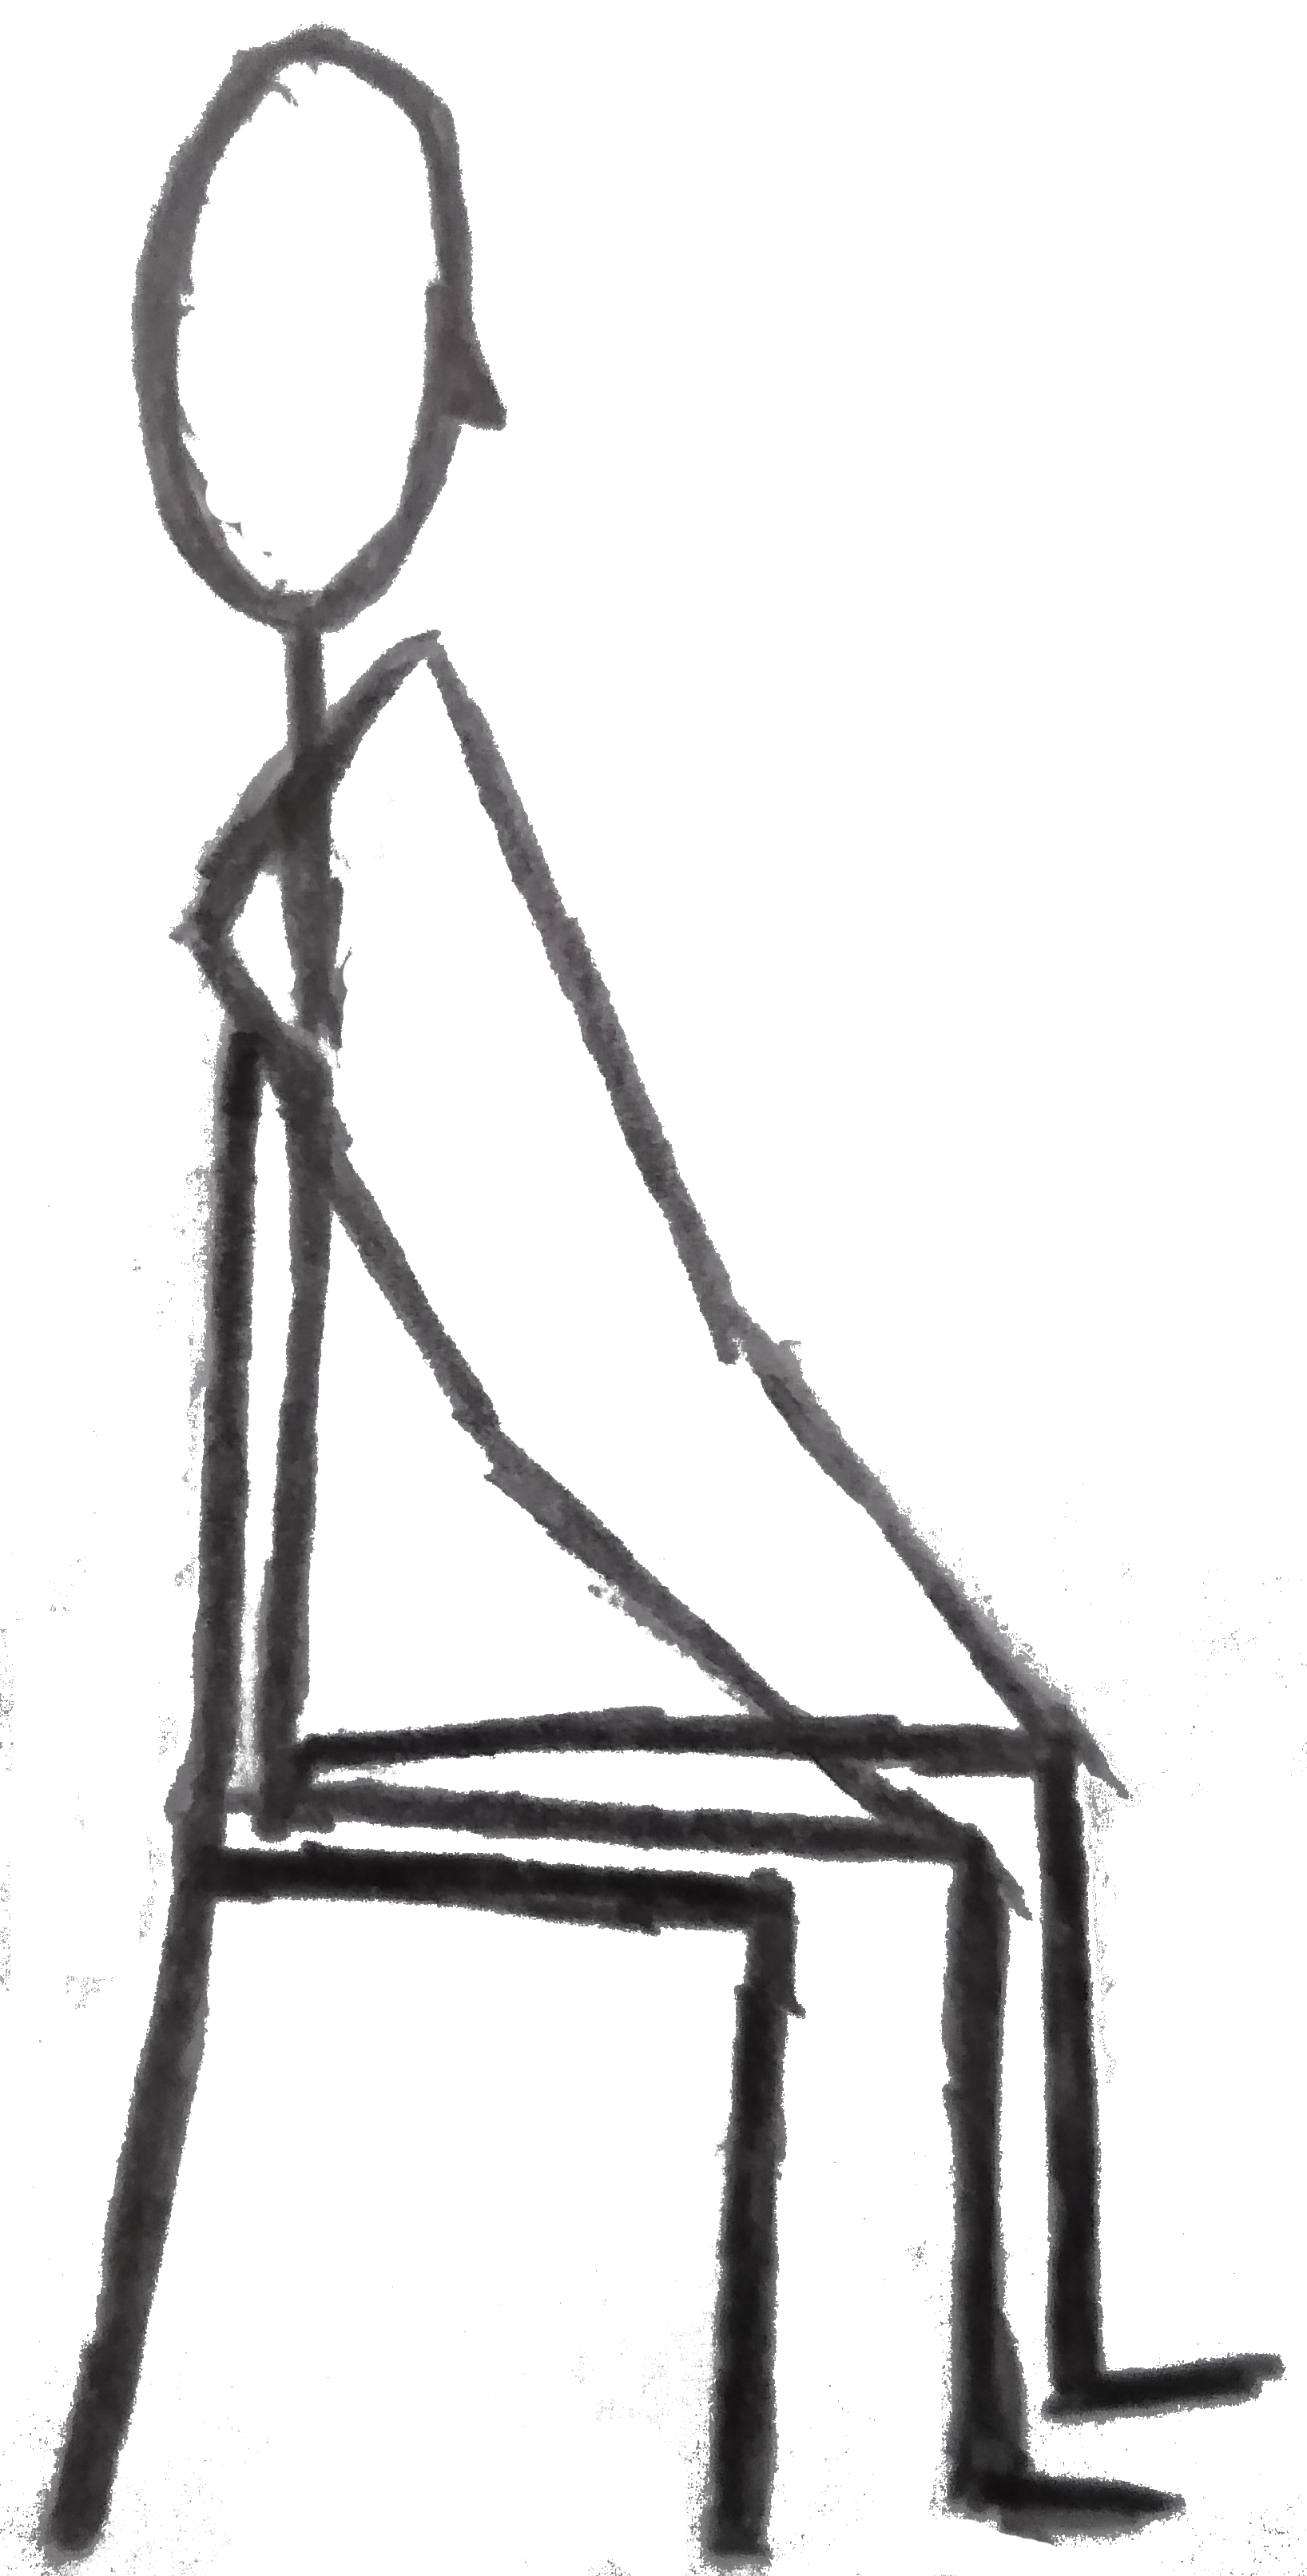
\includegraphics[width=\linewidth]{Sitting_chair_side.png}
%\column{.7\textwidth} % Right column and width
``Autogenous'' means s\structure{elf--generated, independent of outside sources}, --- here a \structure{state of relaxation} ``training'' it's a \structure{progressive process}, while training one gets better.


Autogenous Training AT is a \structure{desensitisation and relaxation method} invented 1932 by  German psychiatrist \structure{Johannes Heinrich Schultz}. Schultz was studying \structure{self--reports of people after being immersed onto a hypnotic state} and he noted that physiological changes are accompanied by certain feelings.

In short, AT works by making suggestions to the body to feel the symptoms accompanied with the relaxation by yourself.
% Write on
%\end{columns}
\end{frame}
%--------------------------------------------------------------------------------------------------------------
\begin{frame}
\frametitle{What is it}
%\begin{columns}[c] % The "c" option specifies centered vertical alignment while the "t" option is used for top vertical alignment

%\column{.3\textwidth} % Left column and width
%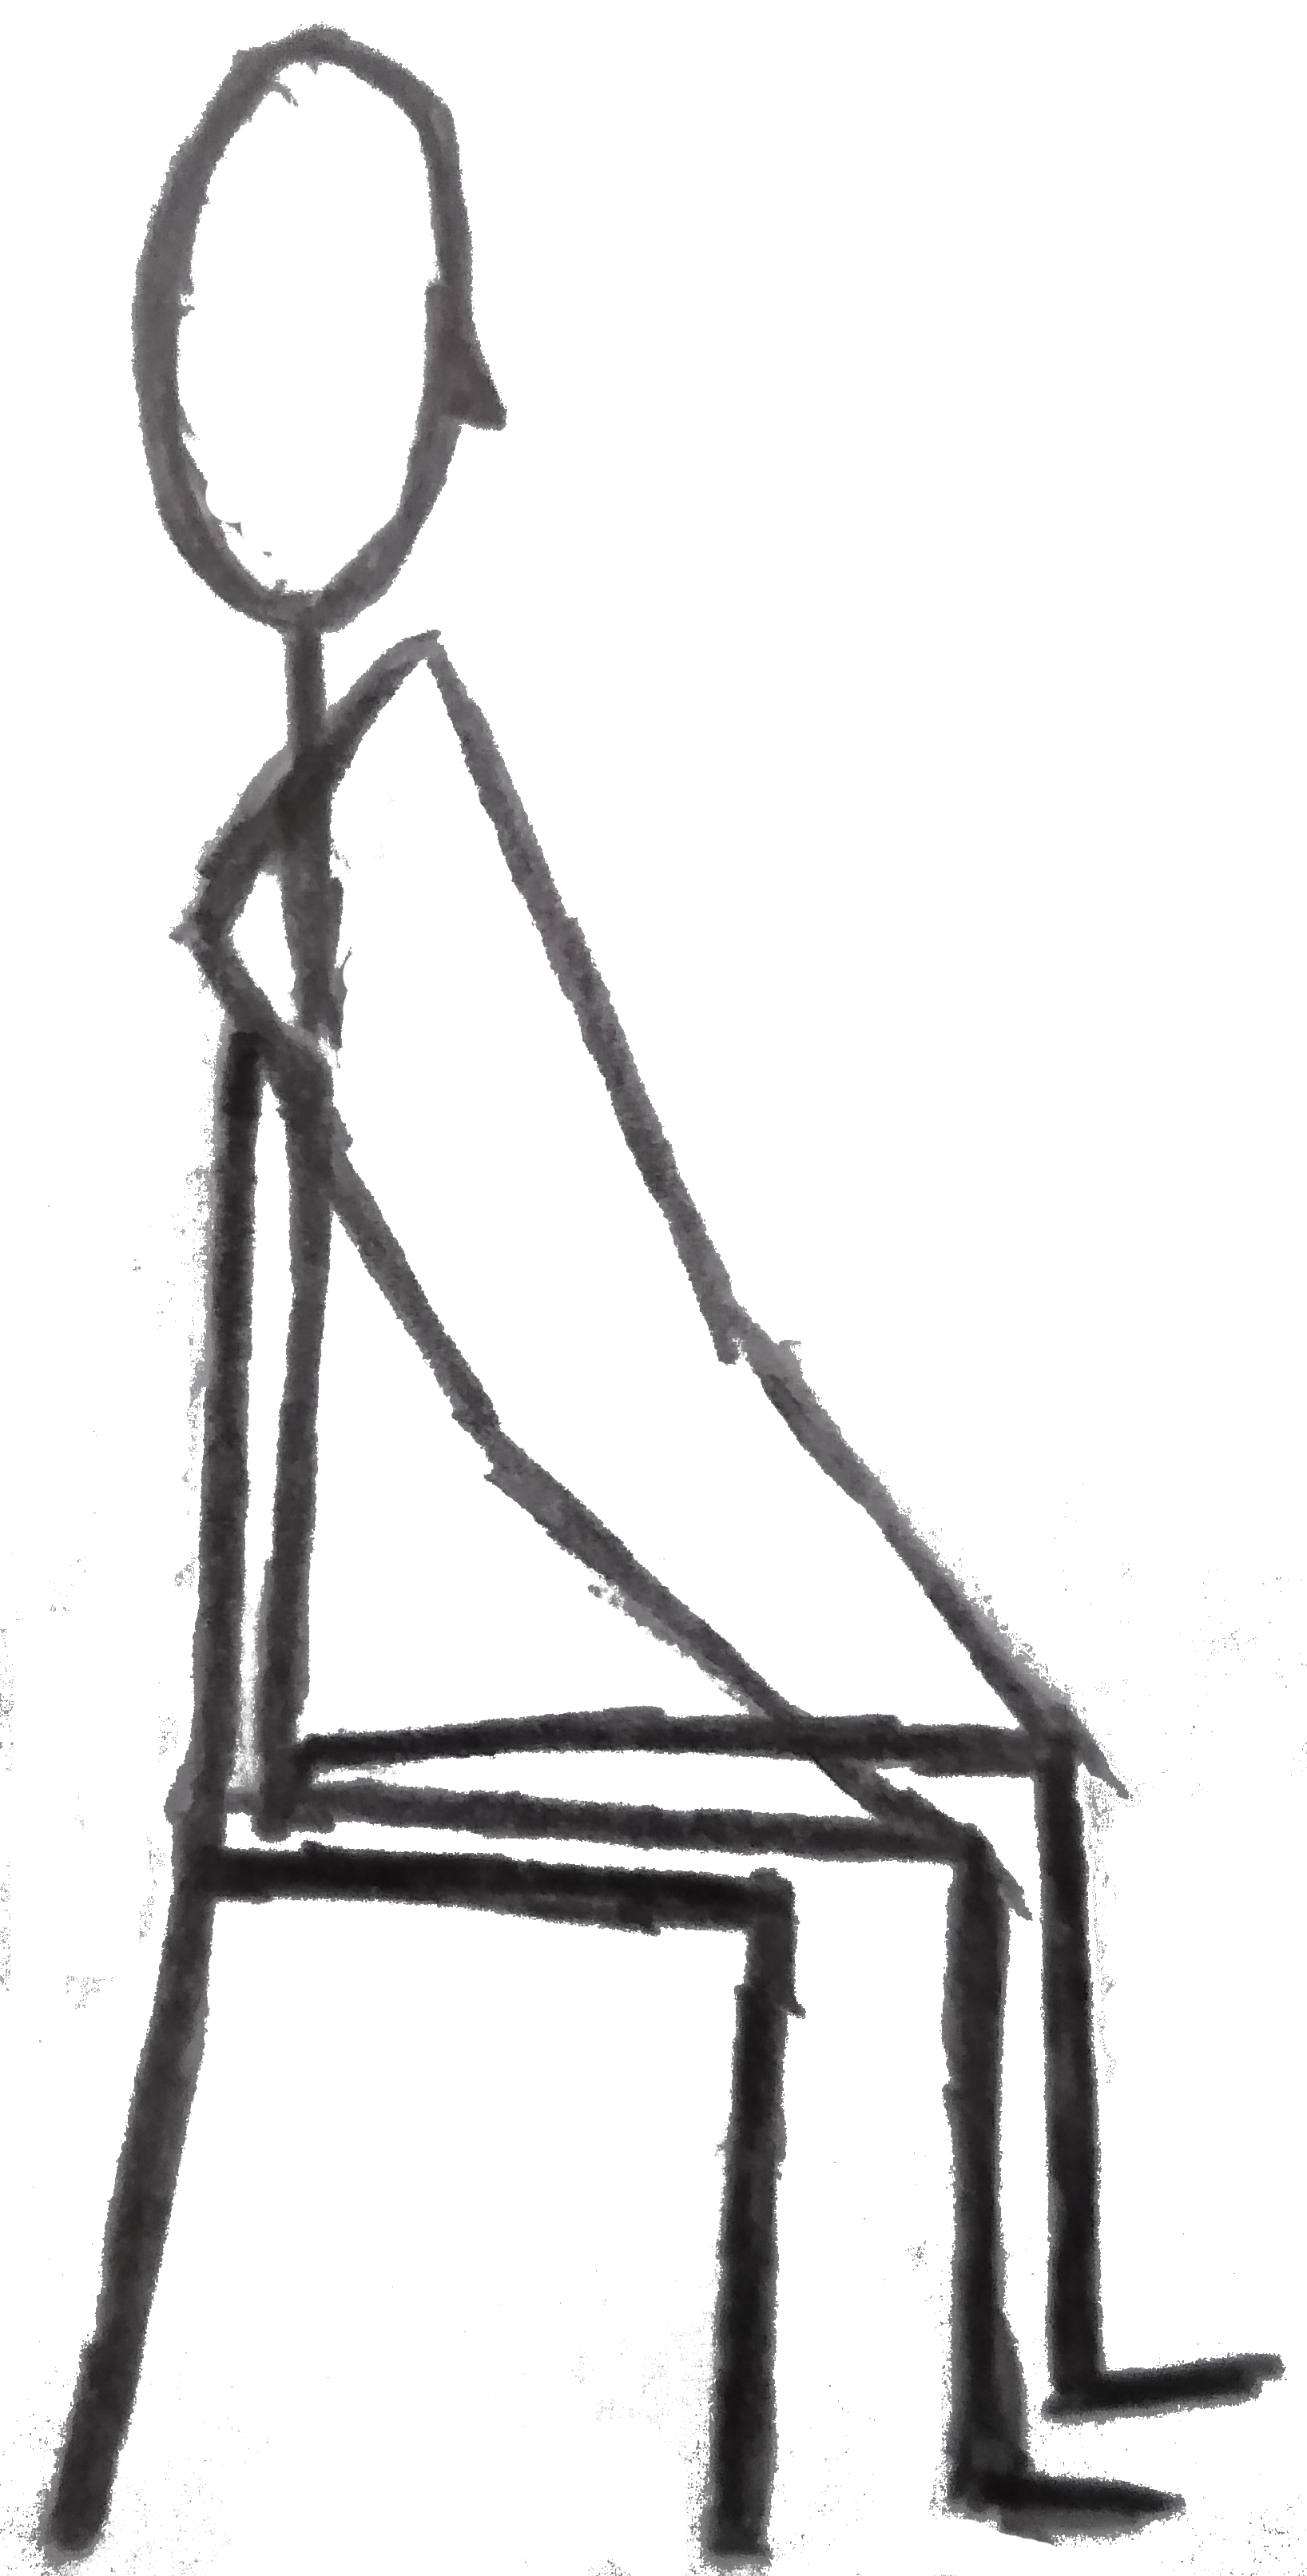
\includegraphics[width=\linewidth]{Sitting_chair_side.png}
%\column{.7\textwidth} % Right column and width
Autogenous Training AT is an \structure{easy to learn and scientific founded self help method}. It \structure{calms and strengthens the mind and psyche} on the detour of the \structure{bodily deep relaxation}. 

AT is in high esteem with doctors, psychologists and pedagogues to help prevent mental and psychosomatic affections.

AT is for the \structure{mind} what \structure{working out} is for the body. It corresponds to our \structure{modern understanding of time}; it only requires 1-2 minutes three times daily in the learning phase. AT is \structure{free of religious or ideological views}.  
% Write on
%\end{columns}
\end{frame}
%--------------------------------------------------------------------------------------------------------------
\begin{frame}
\frametitle{Research on AT}
%\begin{columns}[c] % The "c" option specifies centered vertical alignment while the "t" option is used for top vertical alignment

%\column{.3\textwidth} % Left column and width
%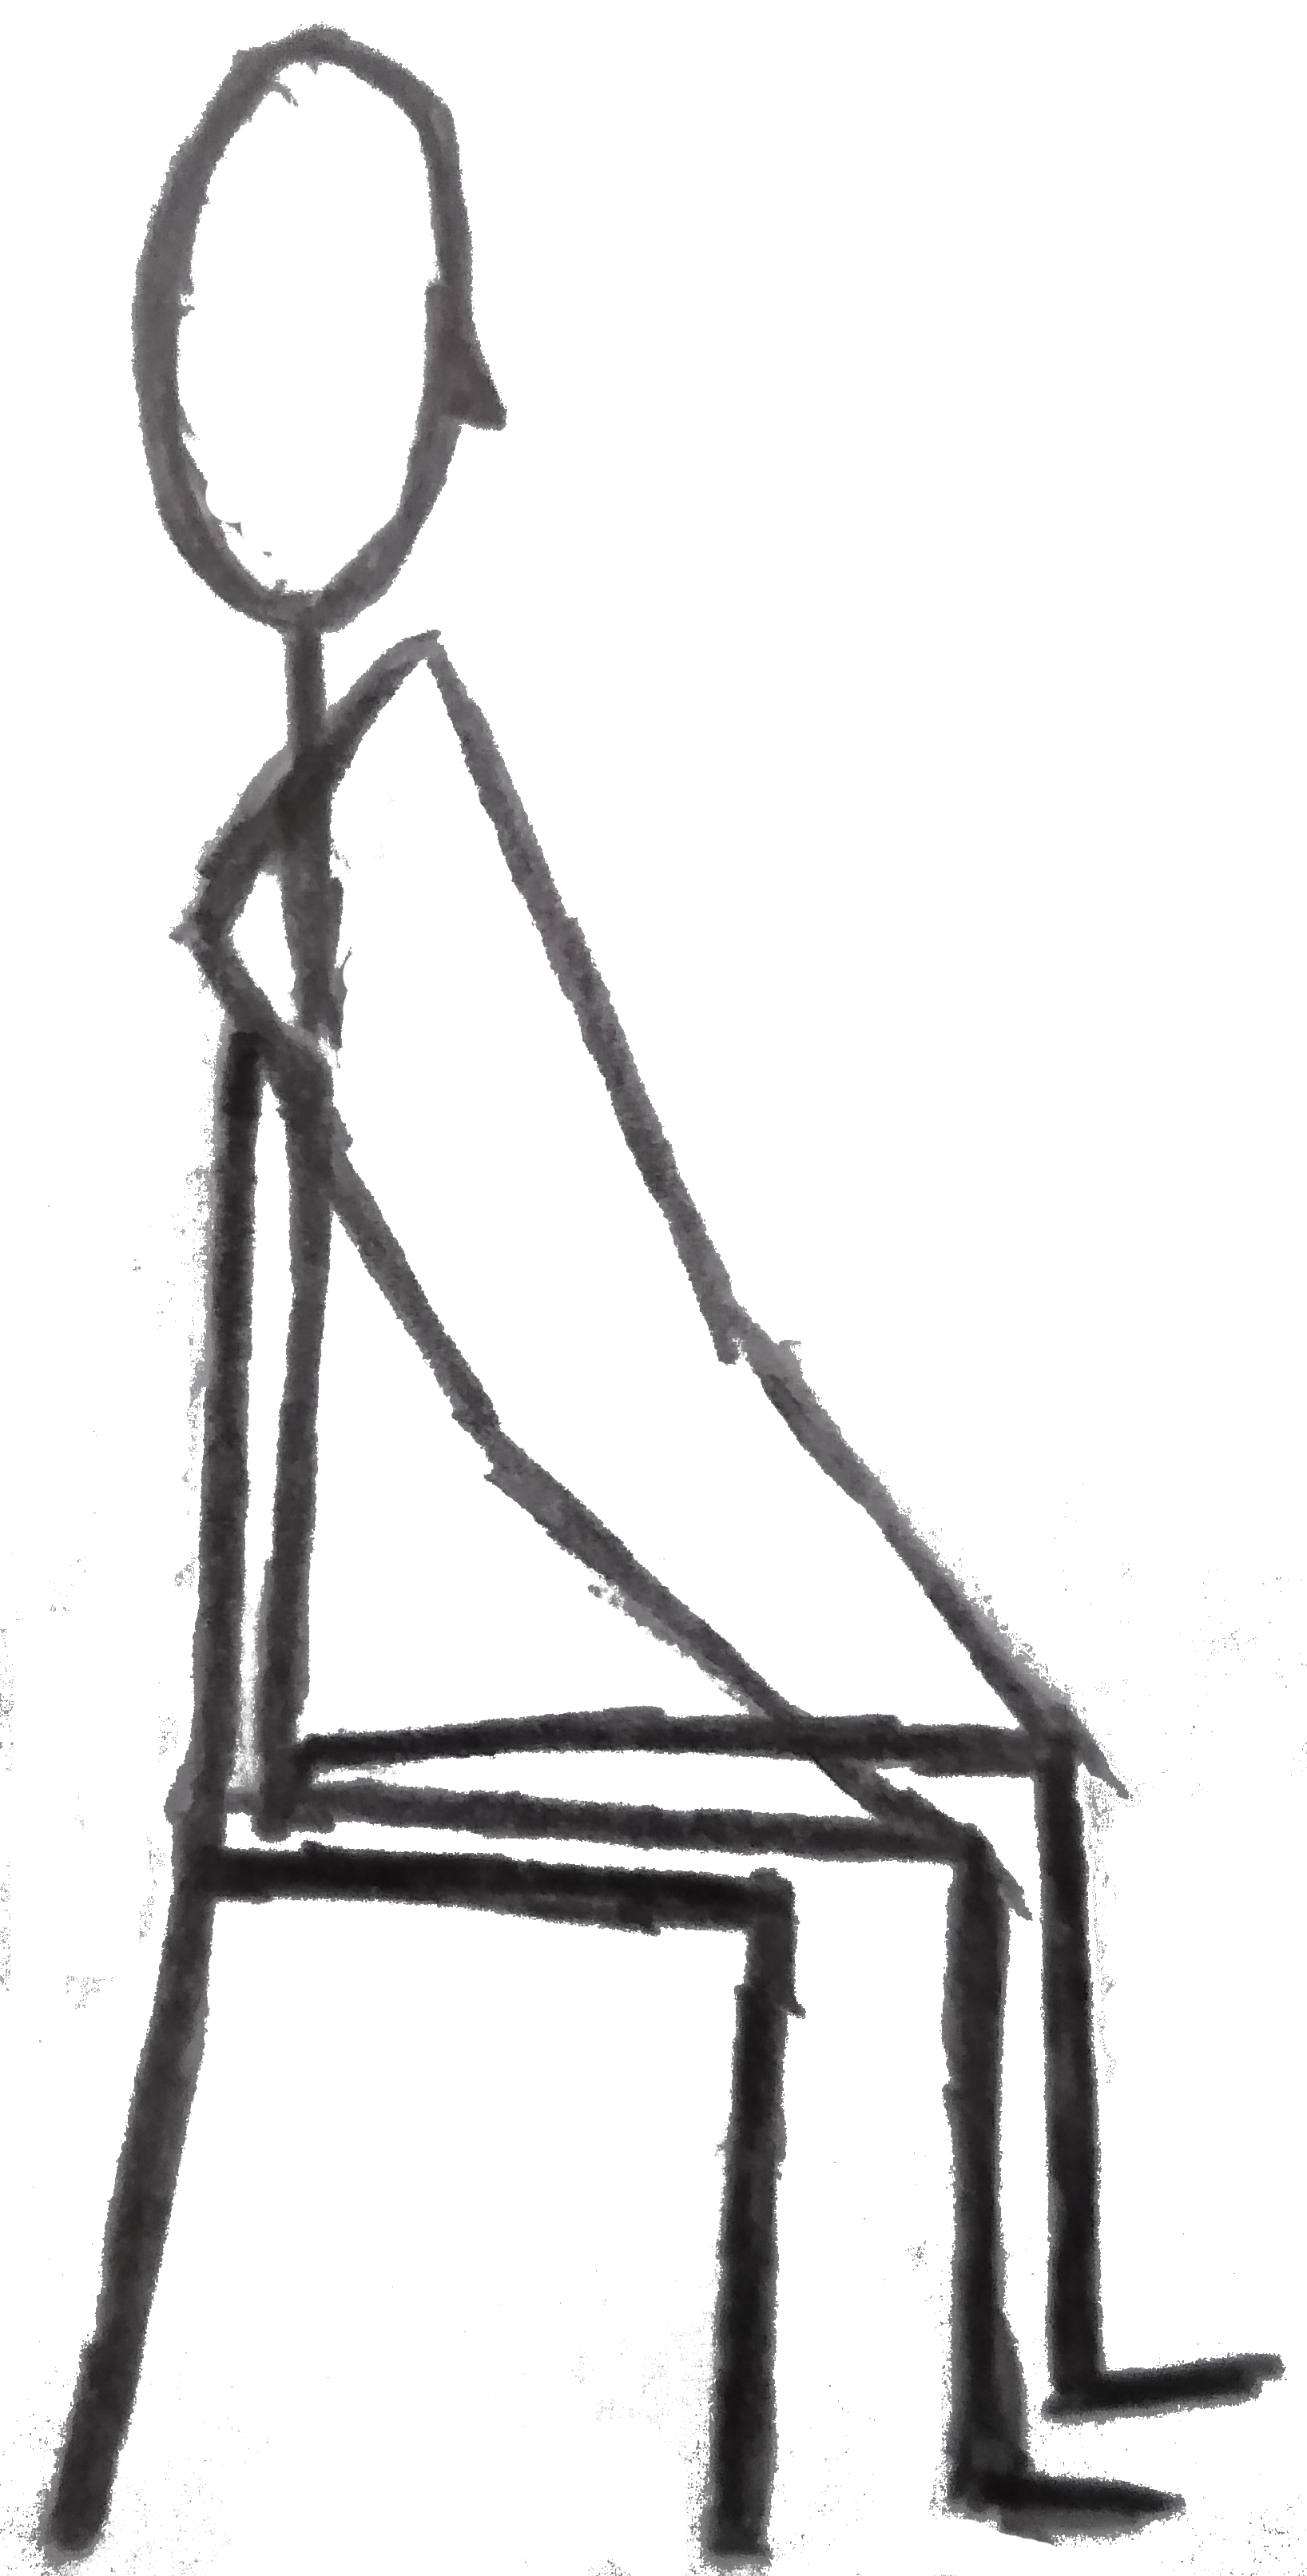
\includegraphics[width=\linewidth]{Sitting_chair_side.png}
%\column{.7\textwidth} % Right column and width
Autogenous Training has been \structure{extensively researched} and the \structure{effects} as well the \structure{mechanism} are well known and documented. This makes autogenous training by now a method which has been \structure{accepted by western medicine} and gets recommended by many physicians. 

We will go in the next slide into the basic \structure{effects} of autogenic training, which are \structure{easily experienced} by the practitioner after starting the training.
% Write on
%\end{columns}
\end{frame}
%--------------------------------------------------------------------------------------------------------------

\begin{frame}
\frametitle{Effects}
%\begin{columns}[c] % The "c" option specifies centered vertical alignment while the "t" option is used for top vertical alignment

%\column{.3\textwidth} % Left column and width
%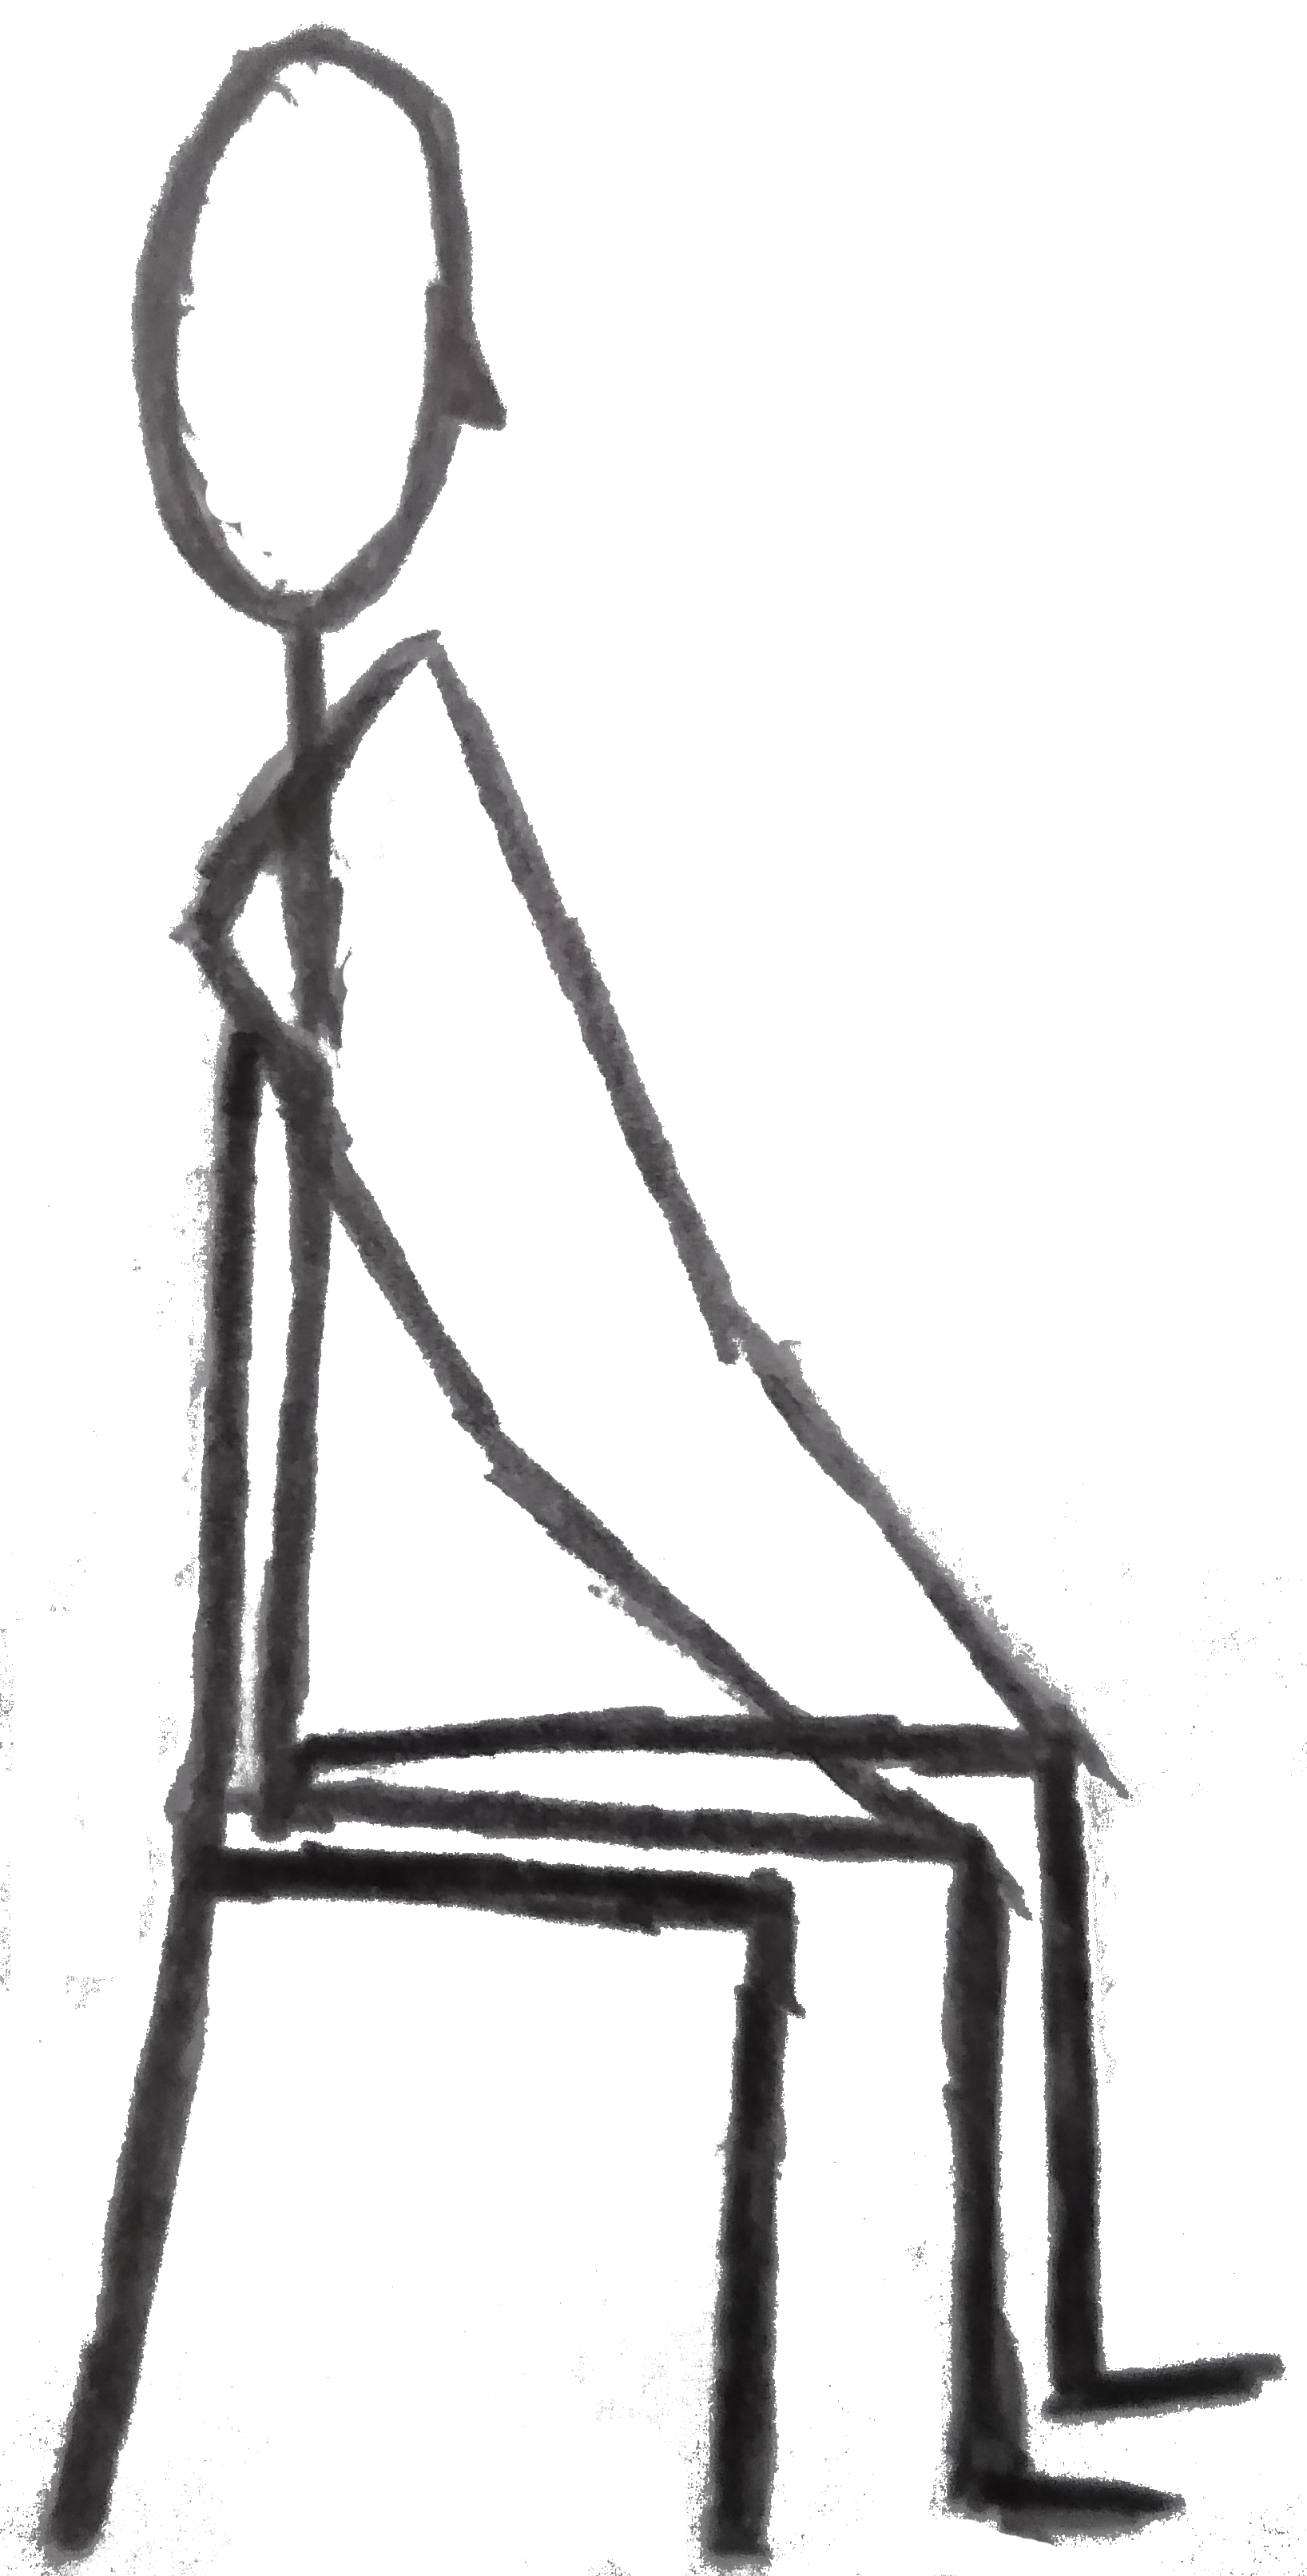
\includegraphics[width=\linewidth]{Sitting_chair_side.png}
%\column{.7\textwidth} % Right column and width
\begin{itemize}
\item[-] Autogenous training is very effective with \structure{stress, anxiety, depression, anger management, insomnia, fatigue and for difficulties with concentration, memory, decision making}. 
\item[-] Quickly \structure{get rid of tiredness} (faster than during normal sleep or passive rest);
\item[-] \structure{Remove mental tension} that results from stress;
\item[-] Influence on range of physiological functions – such as \structure{respiration rate, heart rate, blood supply to individual body parts};
\item[-] \structure{Develop} existing psychological ability such as \structure{thinking, memory, attention}, etc.;
\item[-] \structure{Effectively mobilize physical ability} in sports, it is easy to deal with physical pain.
\end{itemize}

%\end{columns}
\end{frame}
%--------------------------------------------------------------------------------------------------------------

\begin{frame}
\frametitle{Side effects}
%\begin{columns}[c] % The "c" option specifies centered vertical alignment while the "t" option is used for top vertical alignment

%\column{.3\textwidth} % Left column and width
%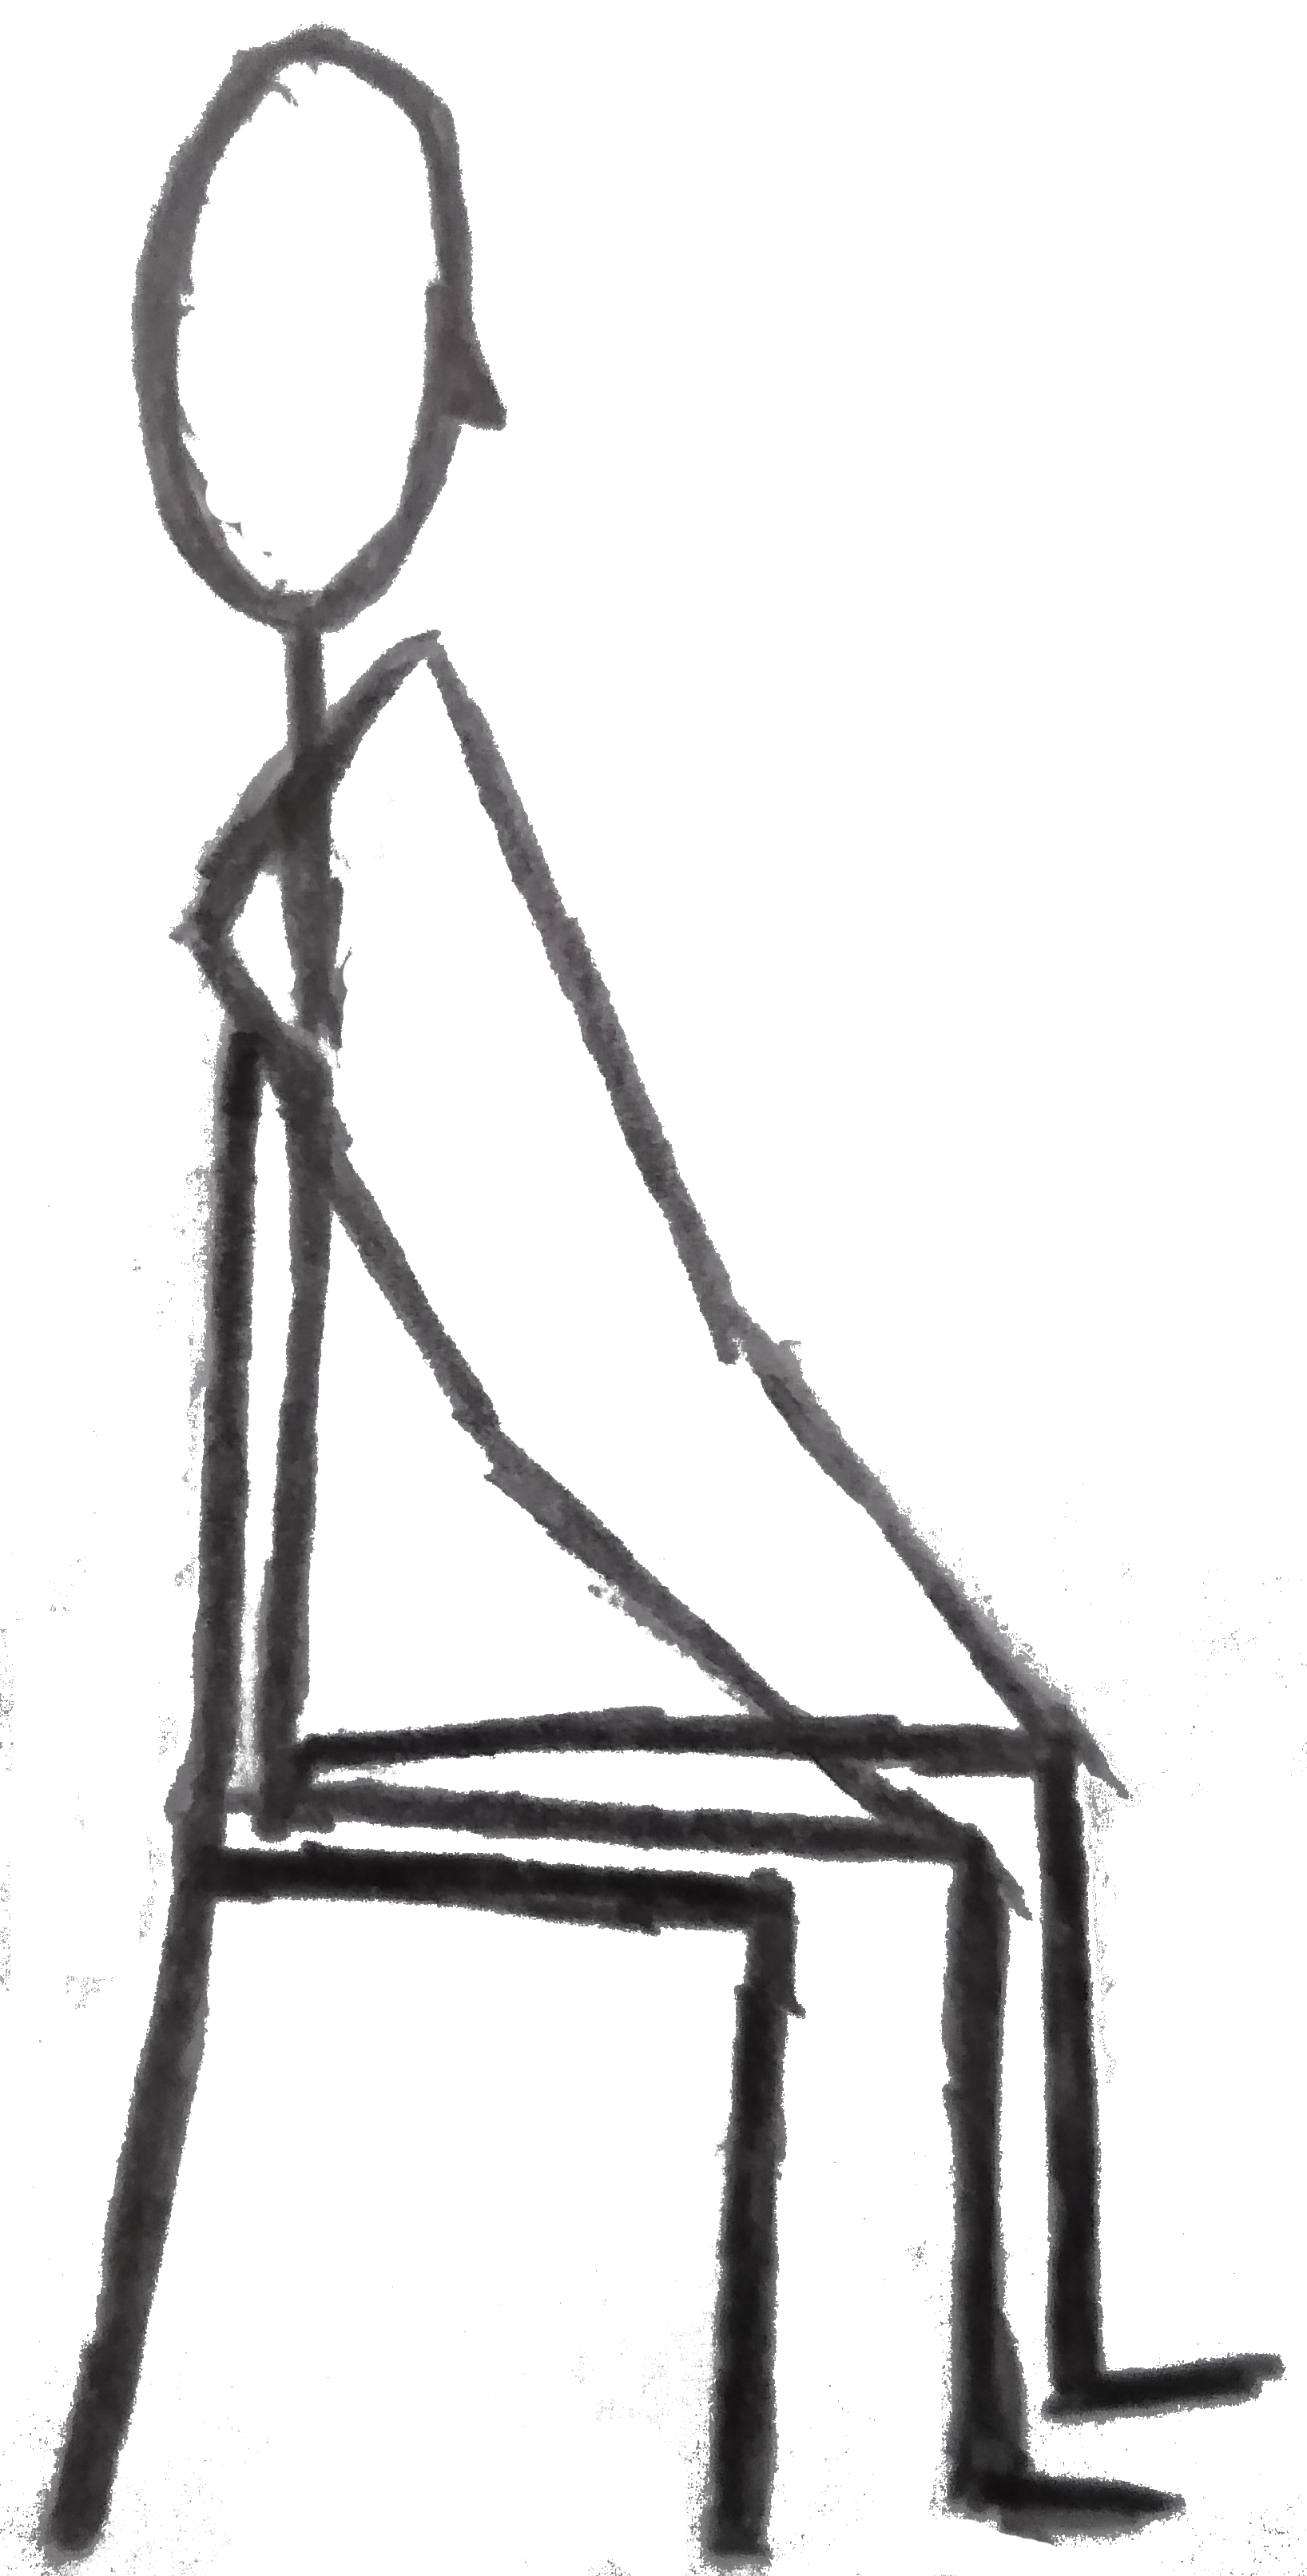
\includegraphics[width=\linewidth]{Sitting_chair_side.png}
%\column{.7\textwidth} % Right column and width
After learning autogenous training from a \structure{qualified source} and with the correct execution, no unwanted side effects will manifest.
If the condition of qualified instruction isn't meet, very \structure{diverse and not controllable side effects} may well occur.


%\end{columns}
\end{frame}
%--------------------------------------------------------------------------------------------------------------
%--------------------------------------------------------------------------------------------------------------

\begin{frame}
\frametitle{Where it is applied}
%\begin{columns}[c] % The "c" option specifies centered vertical alignment while the "t" option is used for top vertical alignment

%\column{.3\textwidth} % Left column and width
%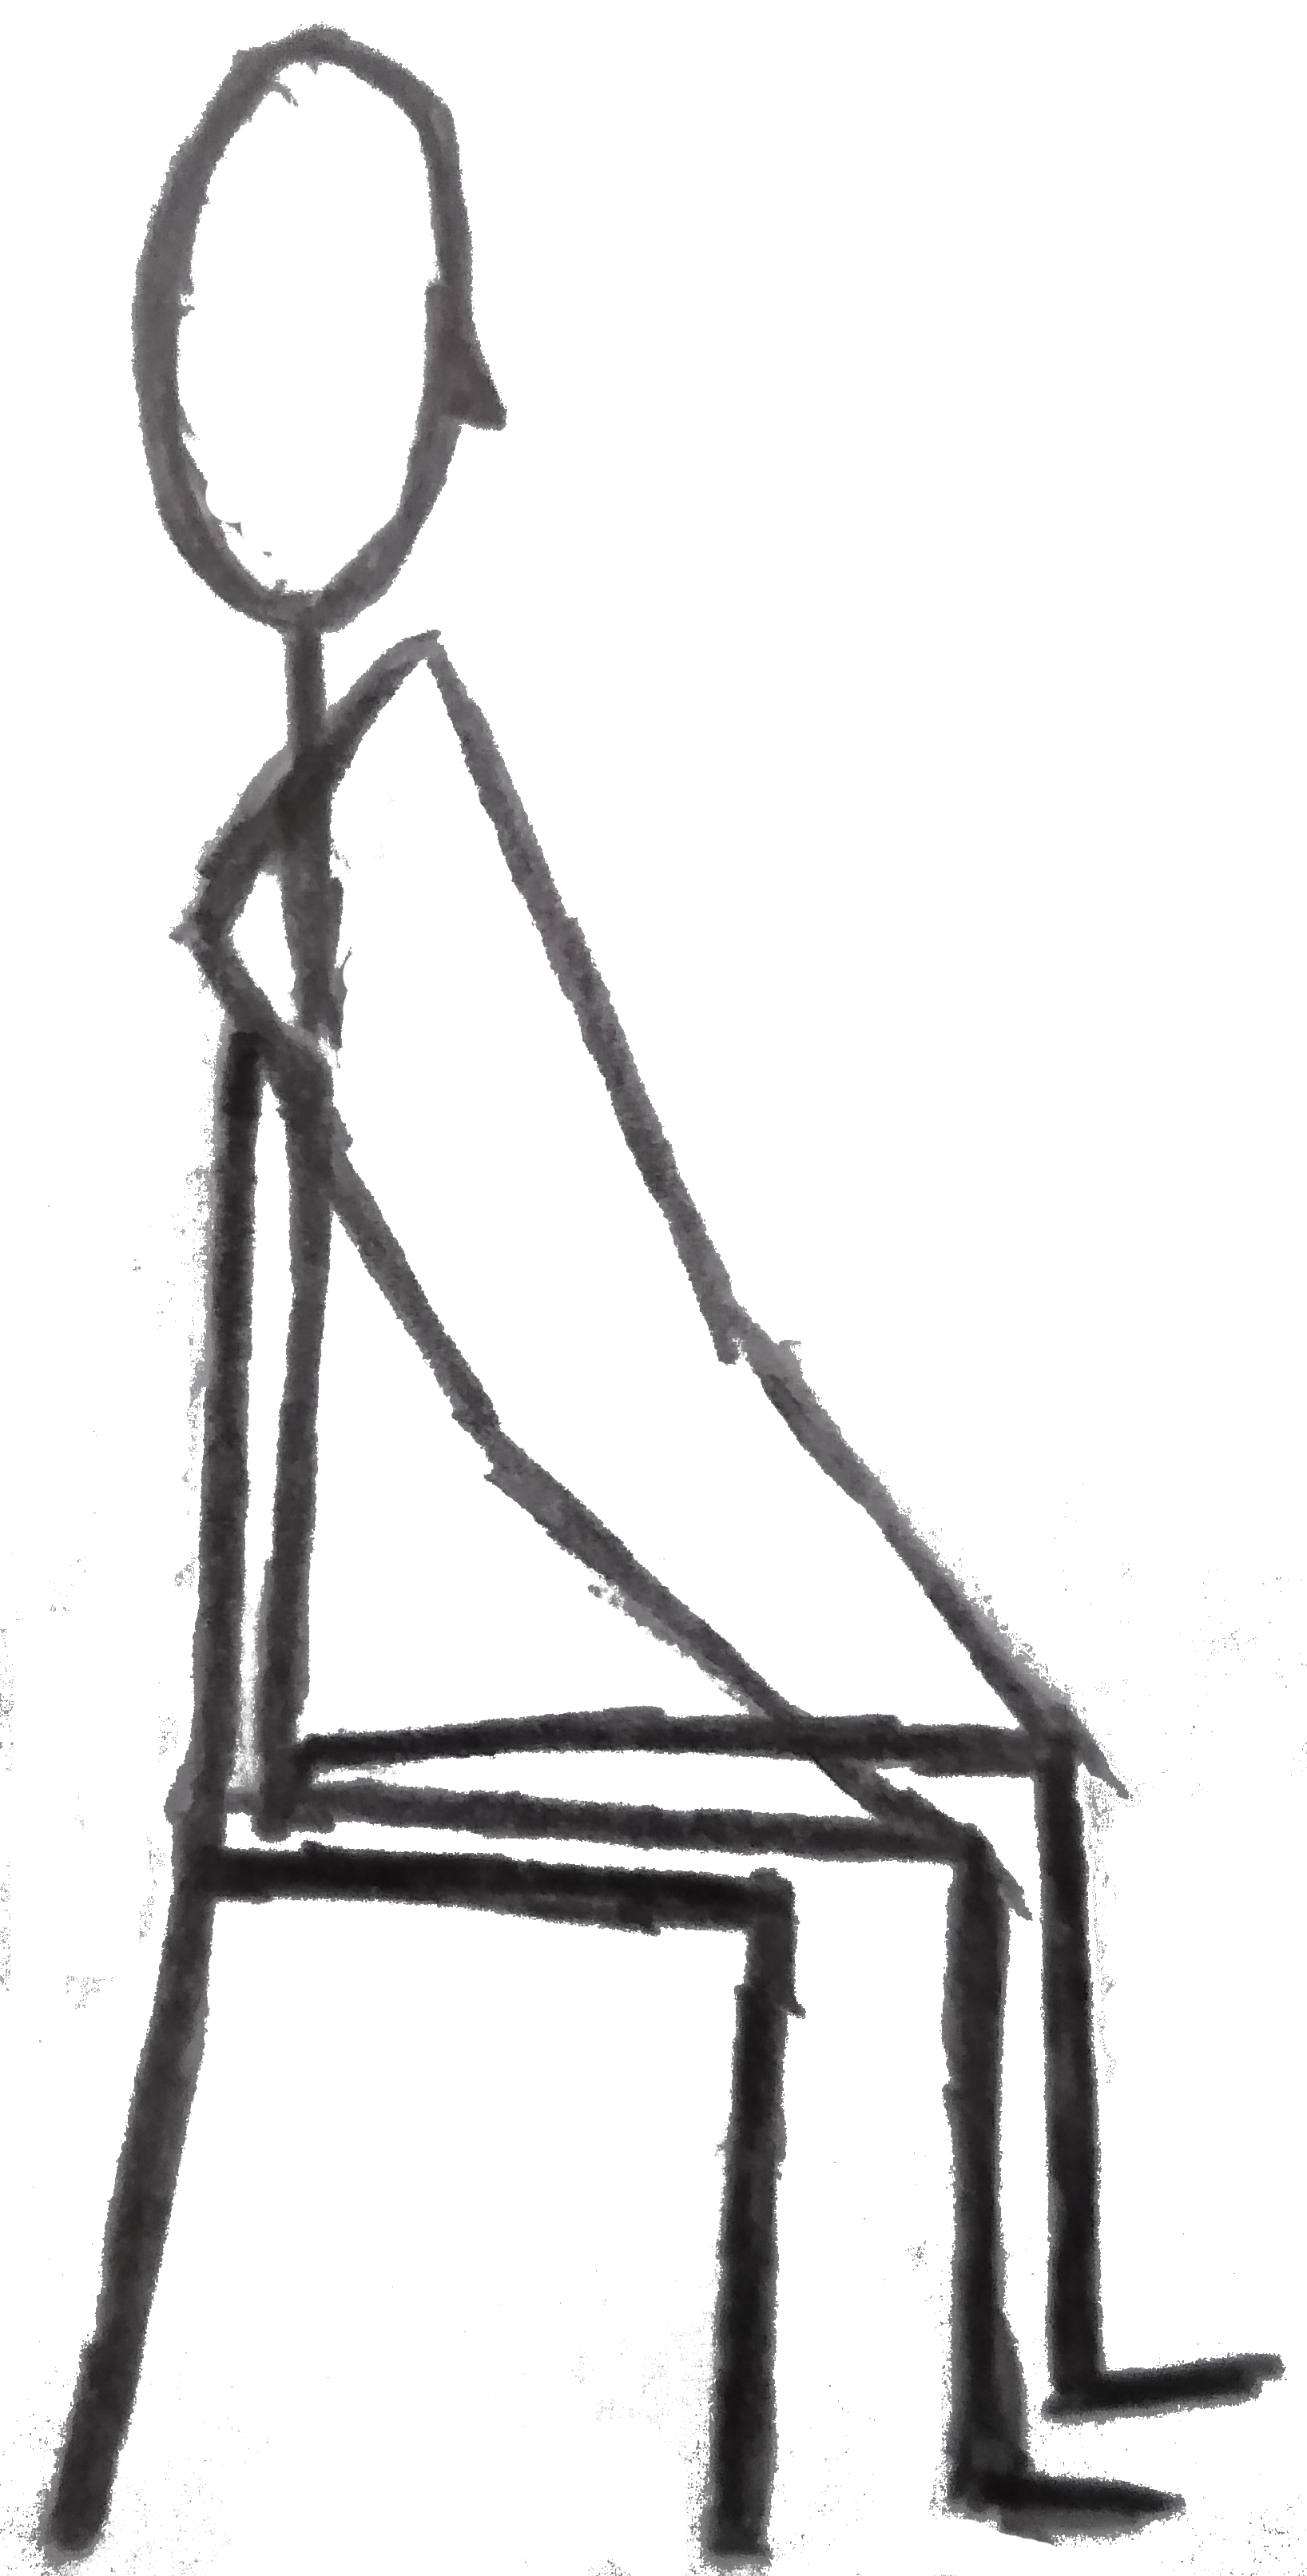
\includegraphics[width=\linewidth]{Sitting_chair_side.png}
%\column{.7\textwidth} % Right column and width
NASA teaches AT to their \structure{astronauts} to help them with the psycho--physiological stressors of space travel. In Japan and Germany, \structure{medical practices teach AT} to assist with the treatment of a wide range of medical complaints. The Autogenous Training Institute of Australia teaches AT for occupational health and safety and has become well known for its work with the \structure{mining, oil and gas industry} as well as \structure{police}. 



%\end{columns}
\end{frame}
%--------------------------------------------------------------------------------------------------------------

\begin{frame}
\frametitle{Progression}
%\begin{columns}[c] % The "c" option specifies centered vertical alignment while the "t" option is used for top vertical alignment

%\column{.3\textwidth} % Left column and width
%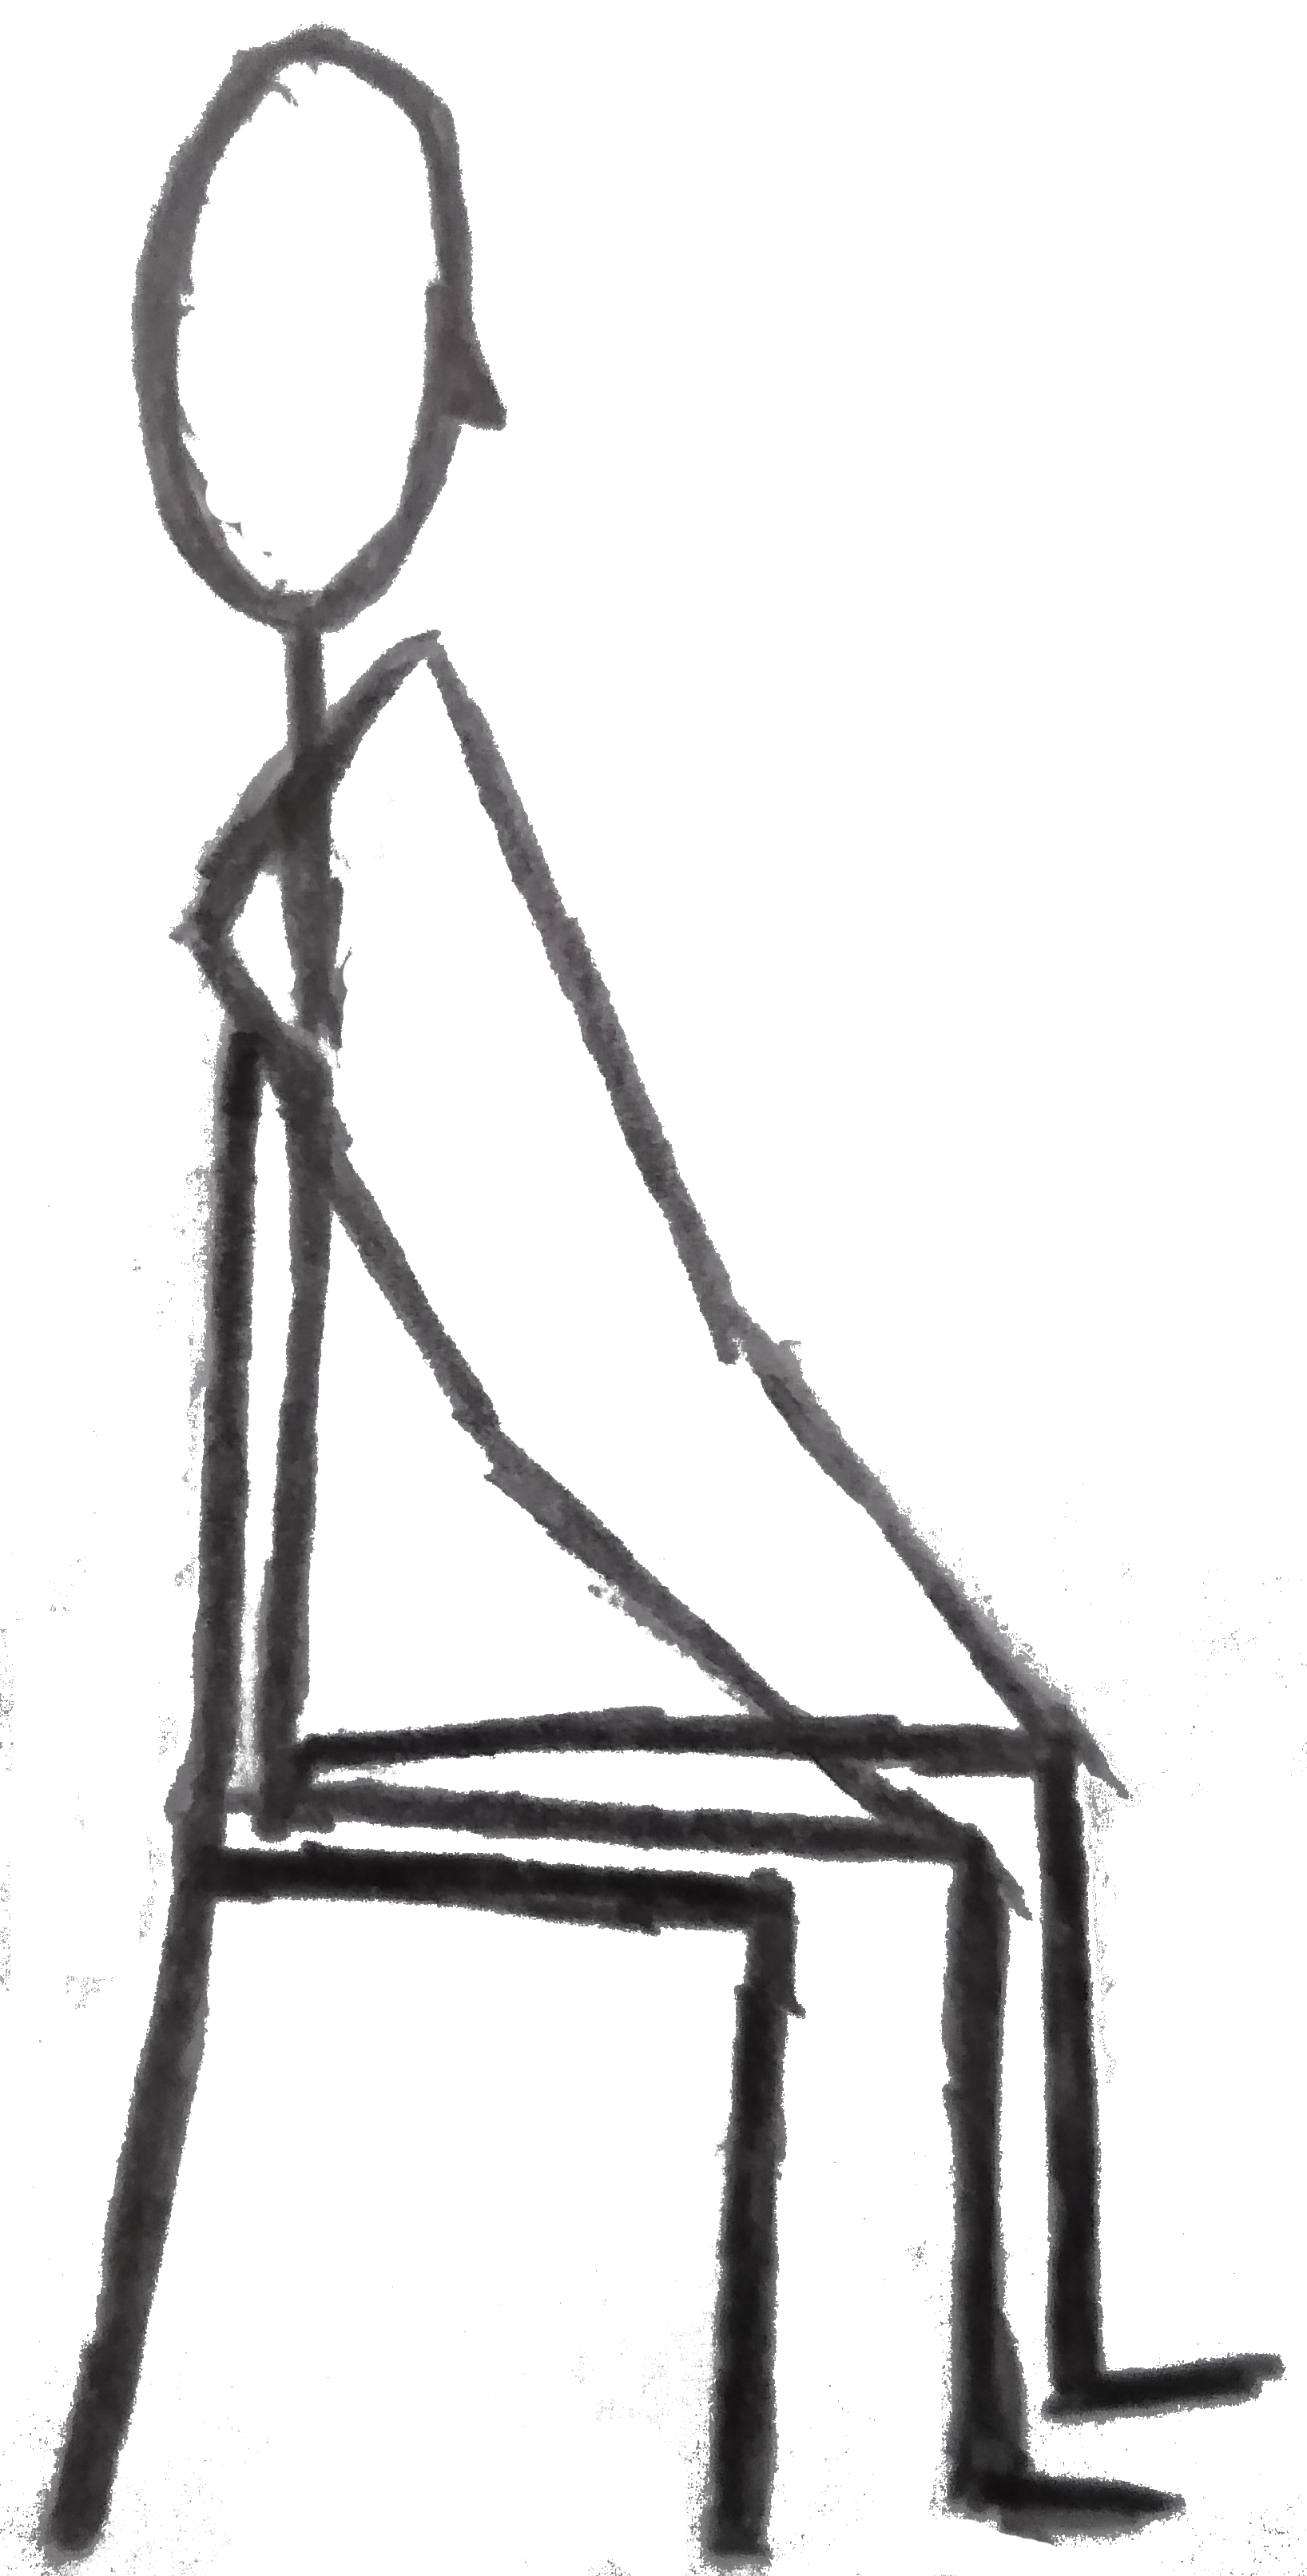
\includegraphics[width=\linewidth]{Sitting_chair_side.png}
%\column{.7\textwidth} % Right column and width

After 6-10 weeks of training, the capacity to switch in a short time too switch from stress to relaxation (reflex) emerges. In that phase, we can add auto suggestions (formula like intentions). Such positive intentions establish themselves in the relaxed state of the autogenous training in the subconscious and get implemented very efficiently.


%\end{columns}
\end{frame}

%--------------------------------------------------------------------------------------------------------------

\begin{frame}
\frametitle{The somatic and the vegetative nervous system}
%\begin{columns}[c] % The "c" option specifies centered vertical alignment while the "t" option is used for top vertical alignment

%\column{.3\textwidth} % Left column and width
%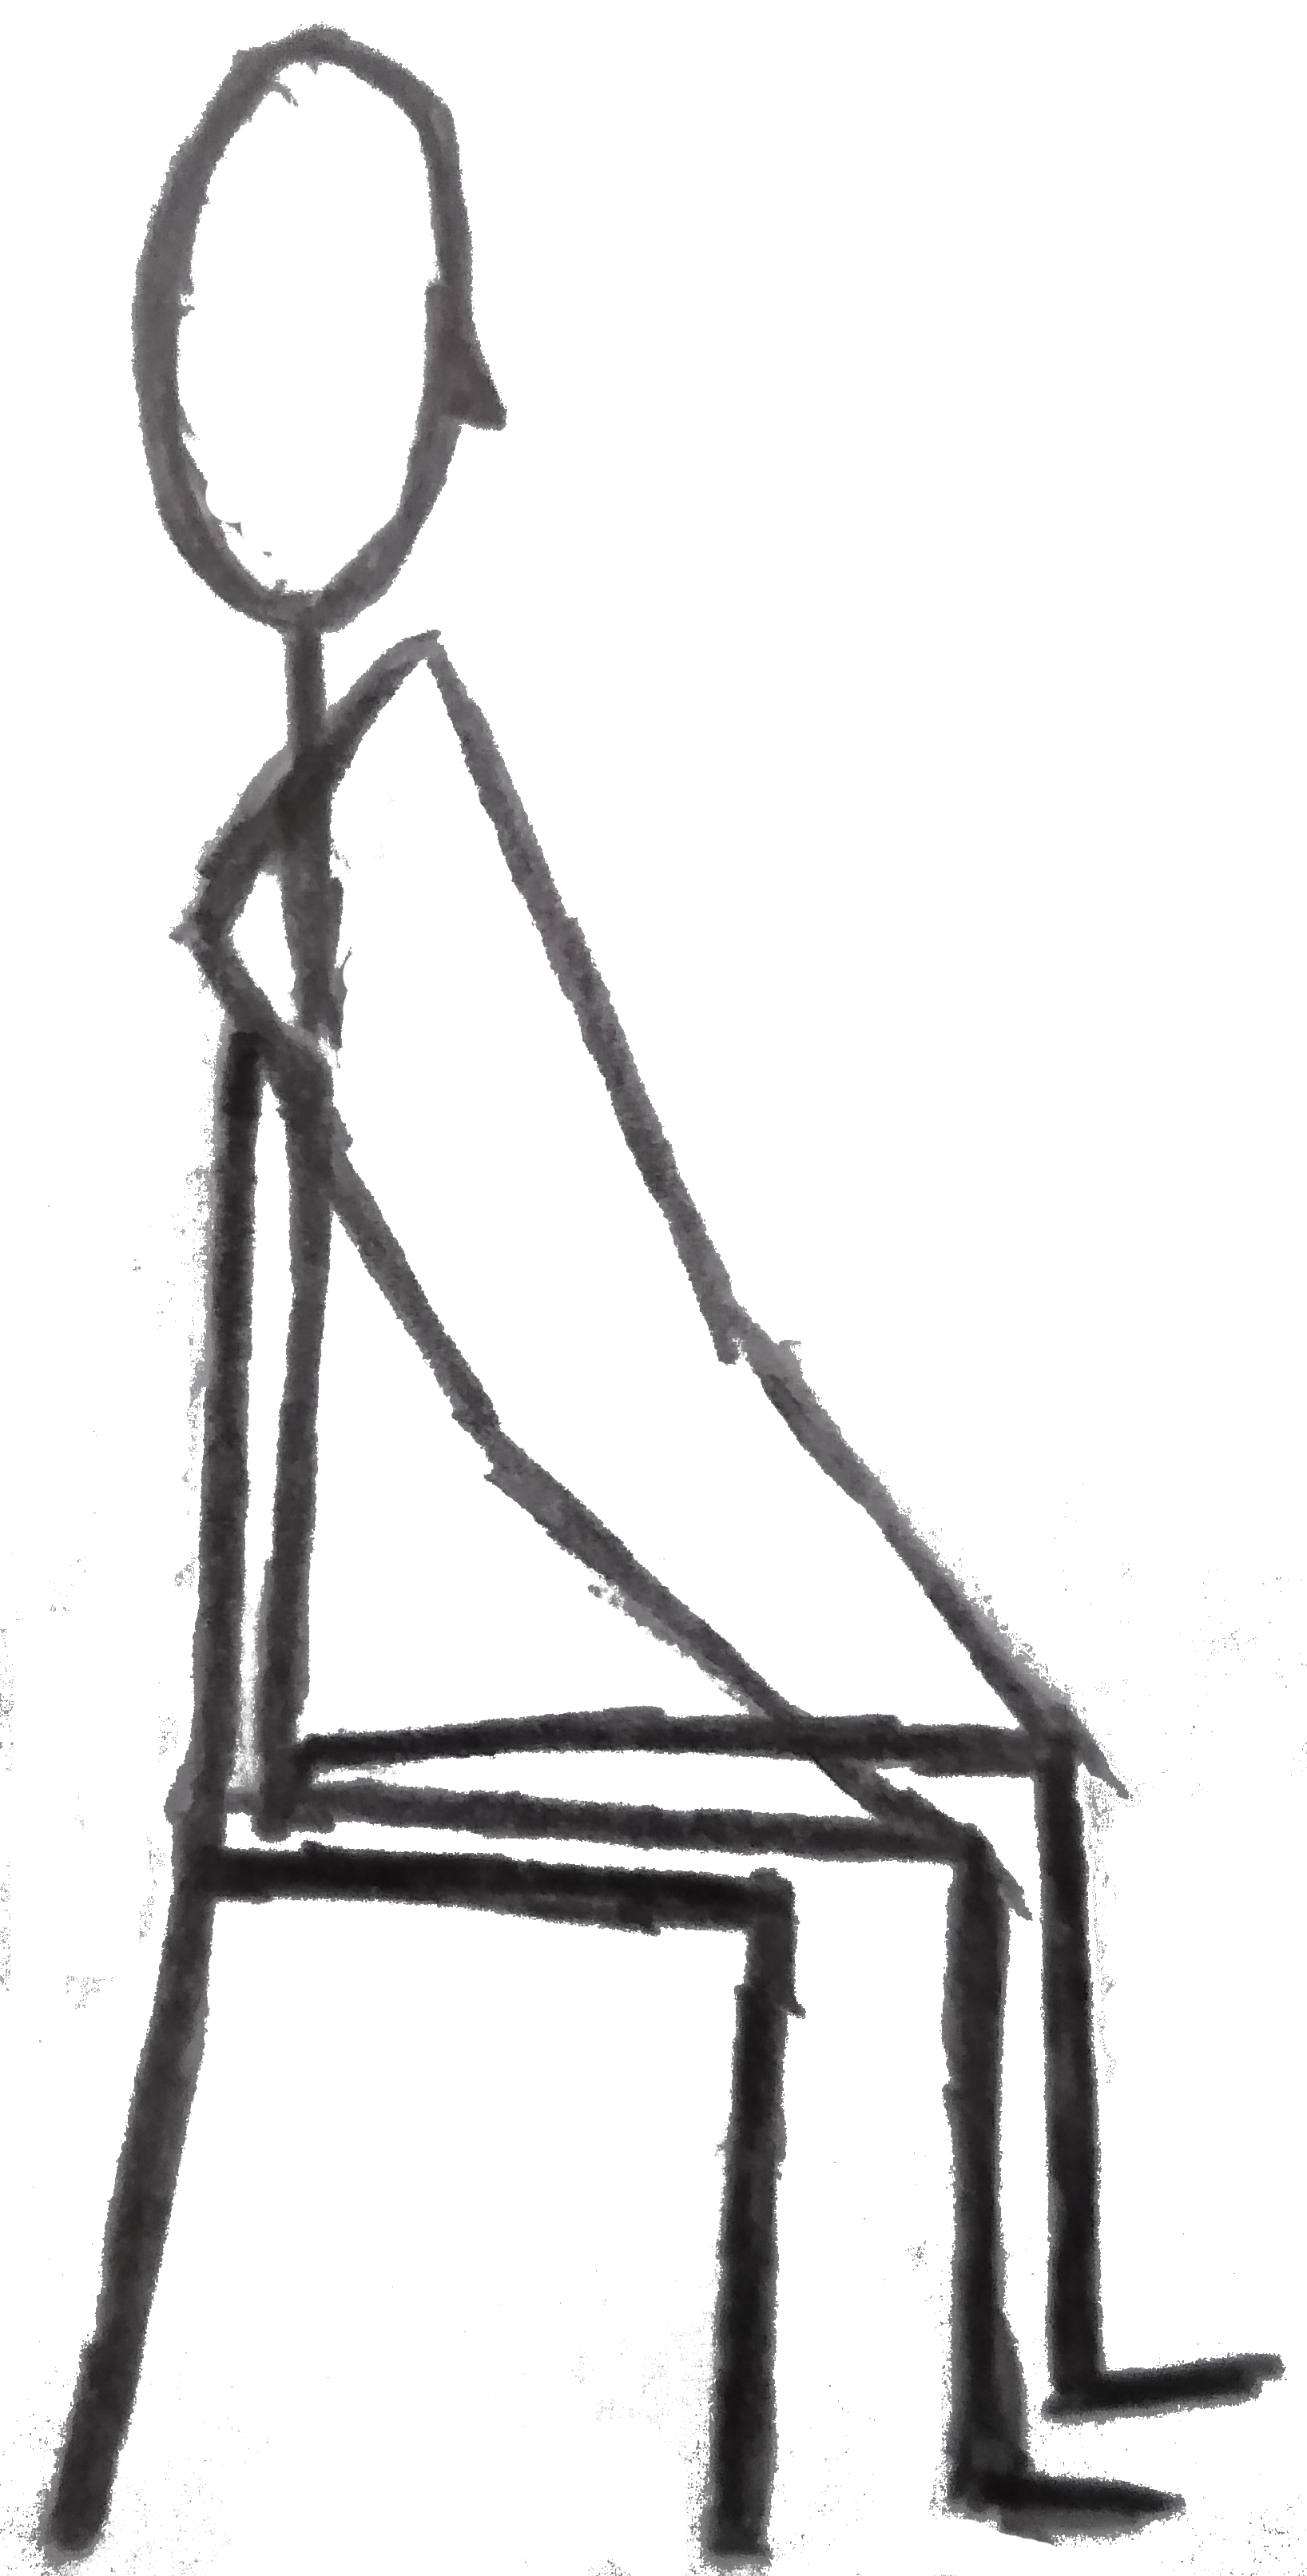
\includegraphics[width=\linewidth]{Sitting_chair_side.png}
%\column{.7\textwidth} % Right column and width

The human body has two nervous systems: the somatic and the vegetative nervous system.

The \structure{somatic nervous system} can be for the most part \structure{controlled consciously}. By the means of the somatic nervous system, a human can coordinate the movement (motor), as \structure{lifting the arm} or curling the little finger.

Another name for the \structure{vegetative} nervous system is the \structure{autonomous nervous system}, because it's actions are mostly except from conscious control. The autonomous nervous system regulates \structure{vital function like breathing, digestion, metabolism, secretion or the water balance} in our body. 
On top of that, the vegetative nervous system controls \structure{organs and organ systems}, as for instance the neuronal control of the sexual organs and the inner eye muscles.


%\end{columns}
\end{frame}

%--------------------------------------------------------------------------------------------------------------

\begin{frame}
\frametitle{The vegetative nervous system}
%\begin{columns}[c] % The "c" option specifies centered vertical alignment while the "t" option is used for top vertical alignment

%\column{.3\textwidth} % Left column and width
%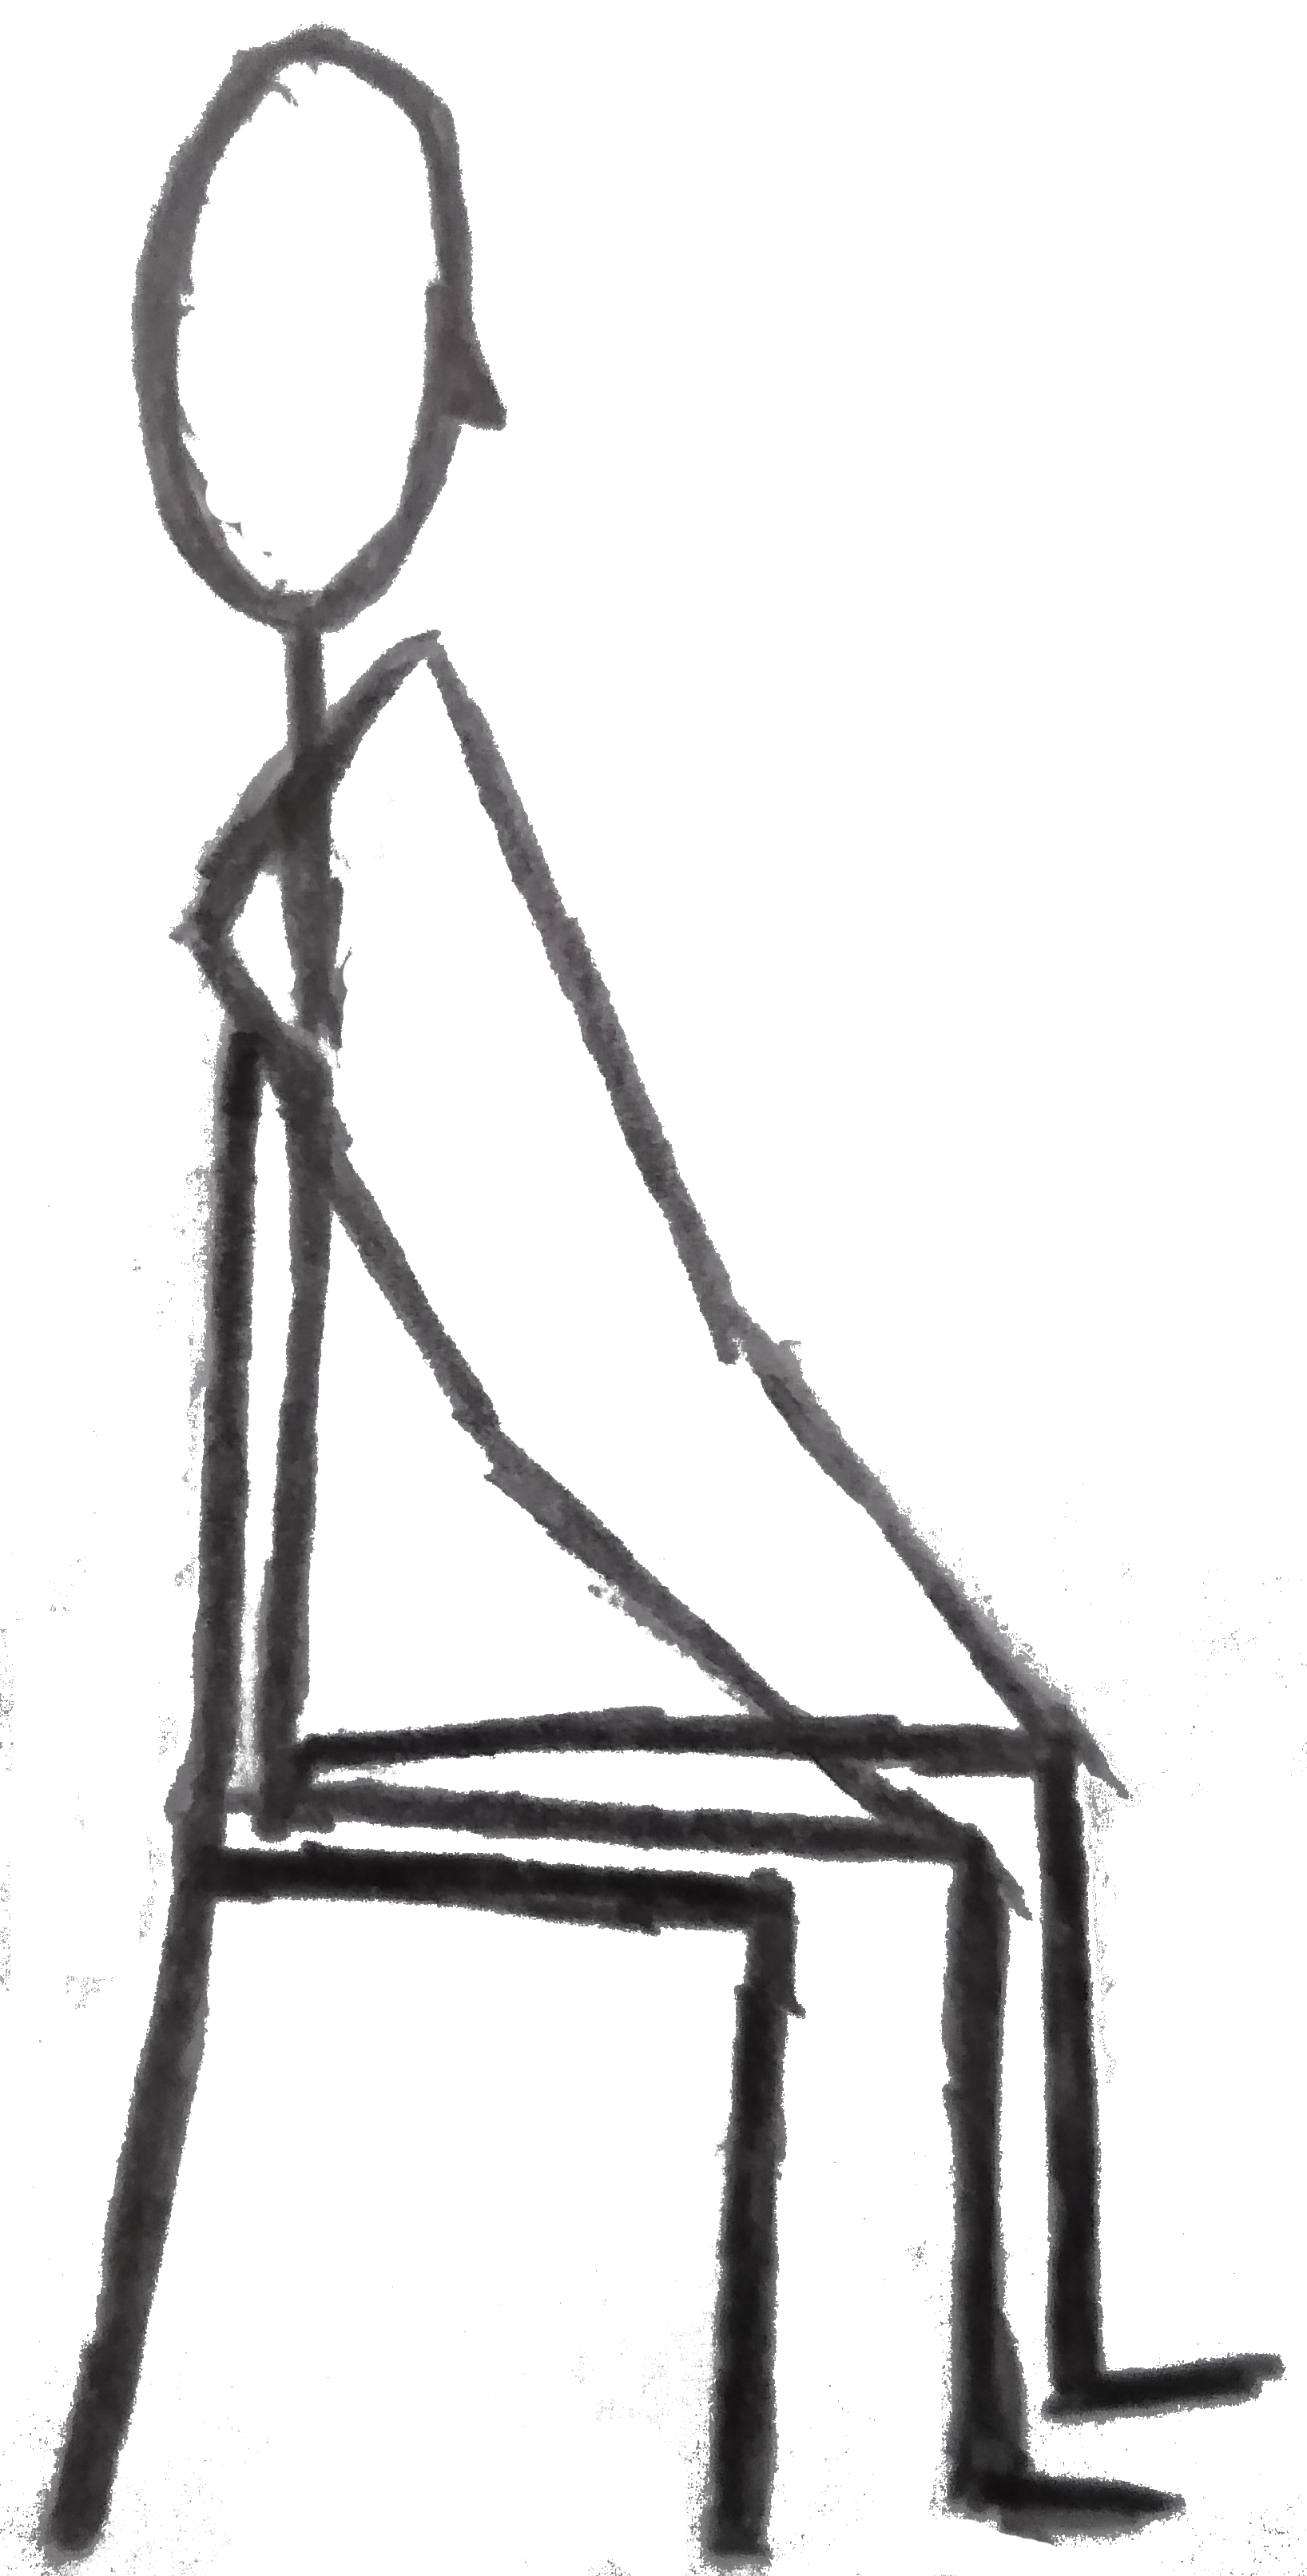
\includegraphics[width=\linewidth]{Sitting_chair_side.png}
%\column{.7\textwidth} % Right column and width

The vegetative nervous system \structure{cannot be controlled consciously}, but can partially \structure{be influenced}, for instance by autogenous training. The vegetative nervous system is even still active in a person lost consciousness.

The vegetative nervous system mainly supplies the so called \structure{smooth muscles} of all \structure{organs, the heart and the glands}. Smooth muscle are in the \structure{organs, which are exempt from conscious control}, as for instance the stomach, colon and pancreas.



%\end{columns}
\end{frame}


%---------------------------------------------------------------
\begin{frame}
\frametitle{Sympathetic, parasympathetic and the enteric nervous system}
%\begin{columns}[c] % The "c" option specifies centered vertical alignment while the "t" option is used for top vertical alignment

%\column{.3\textwidth} % Left column and width
%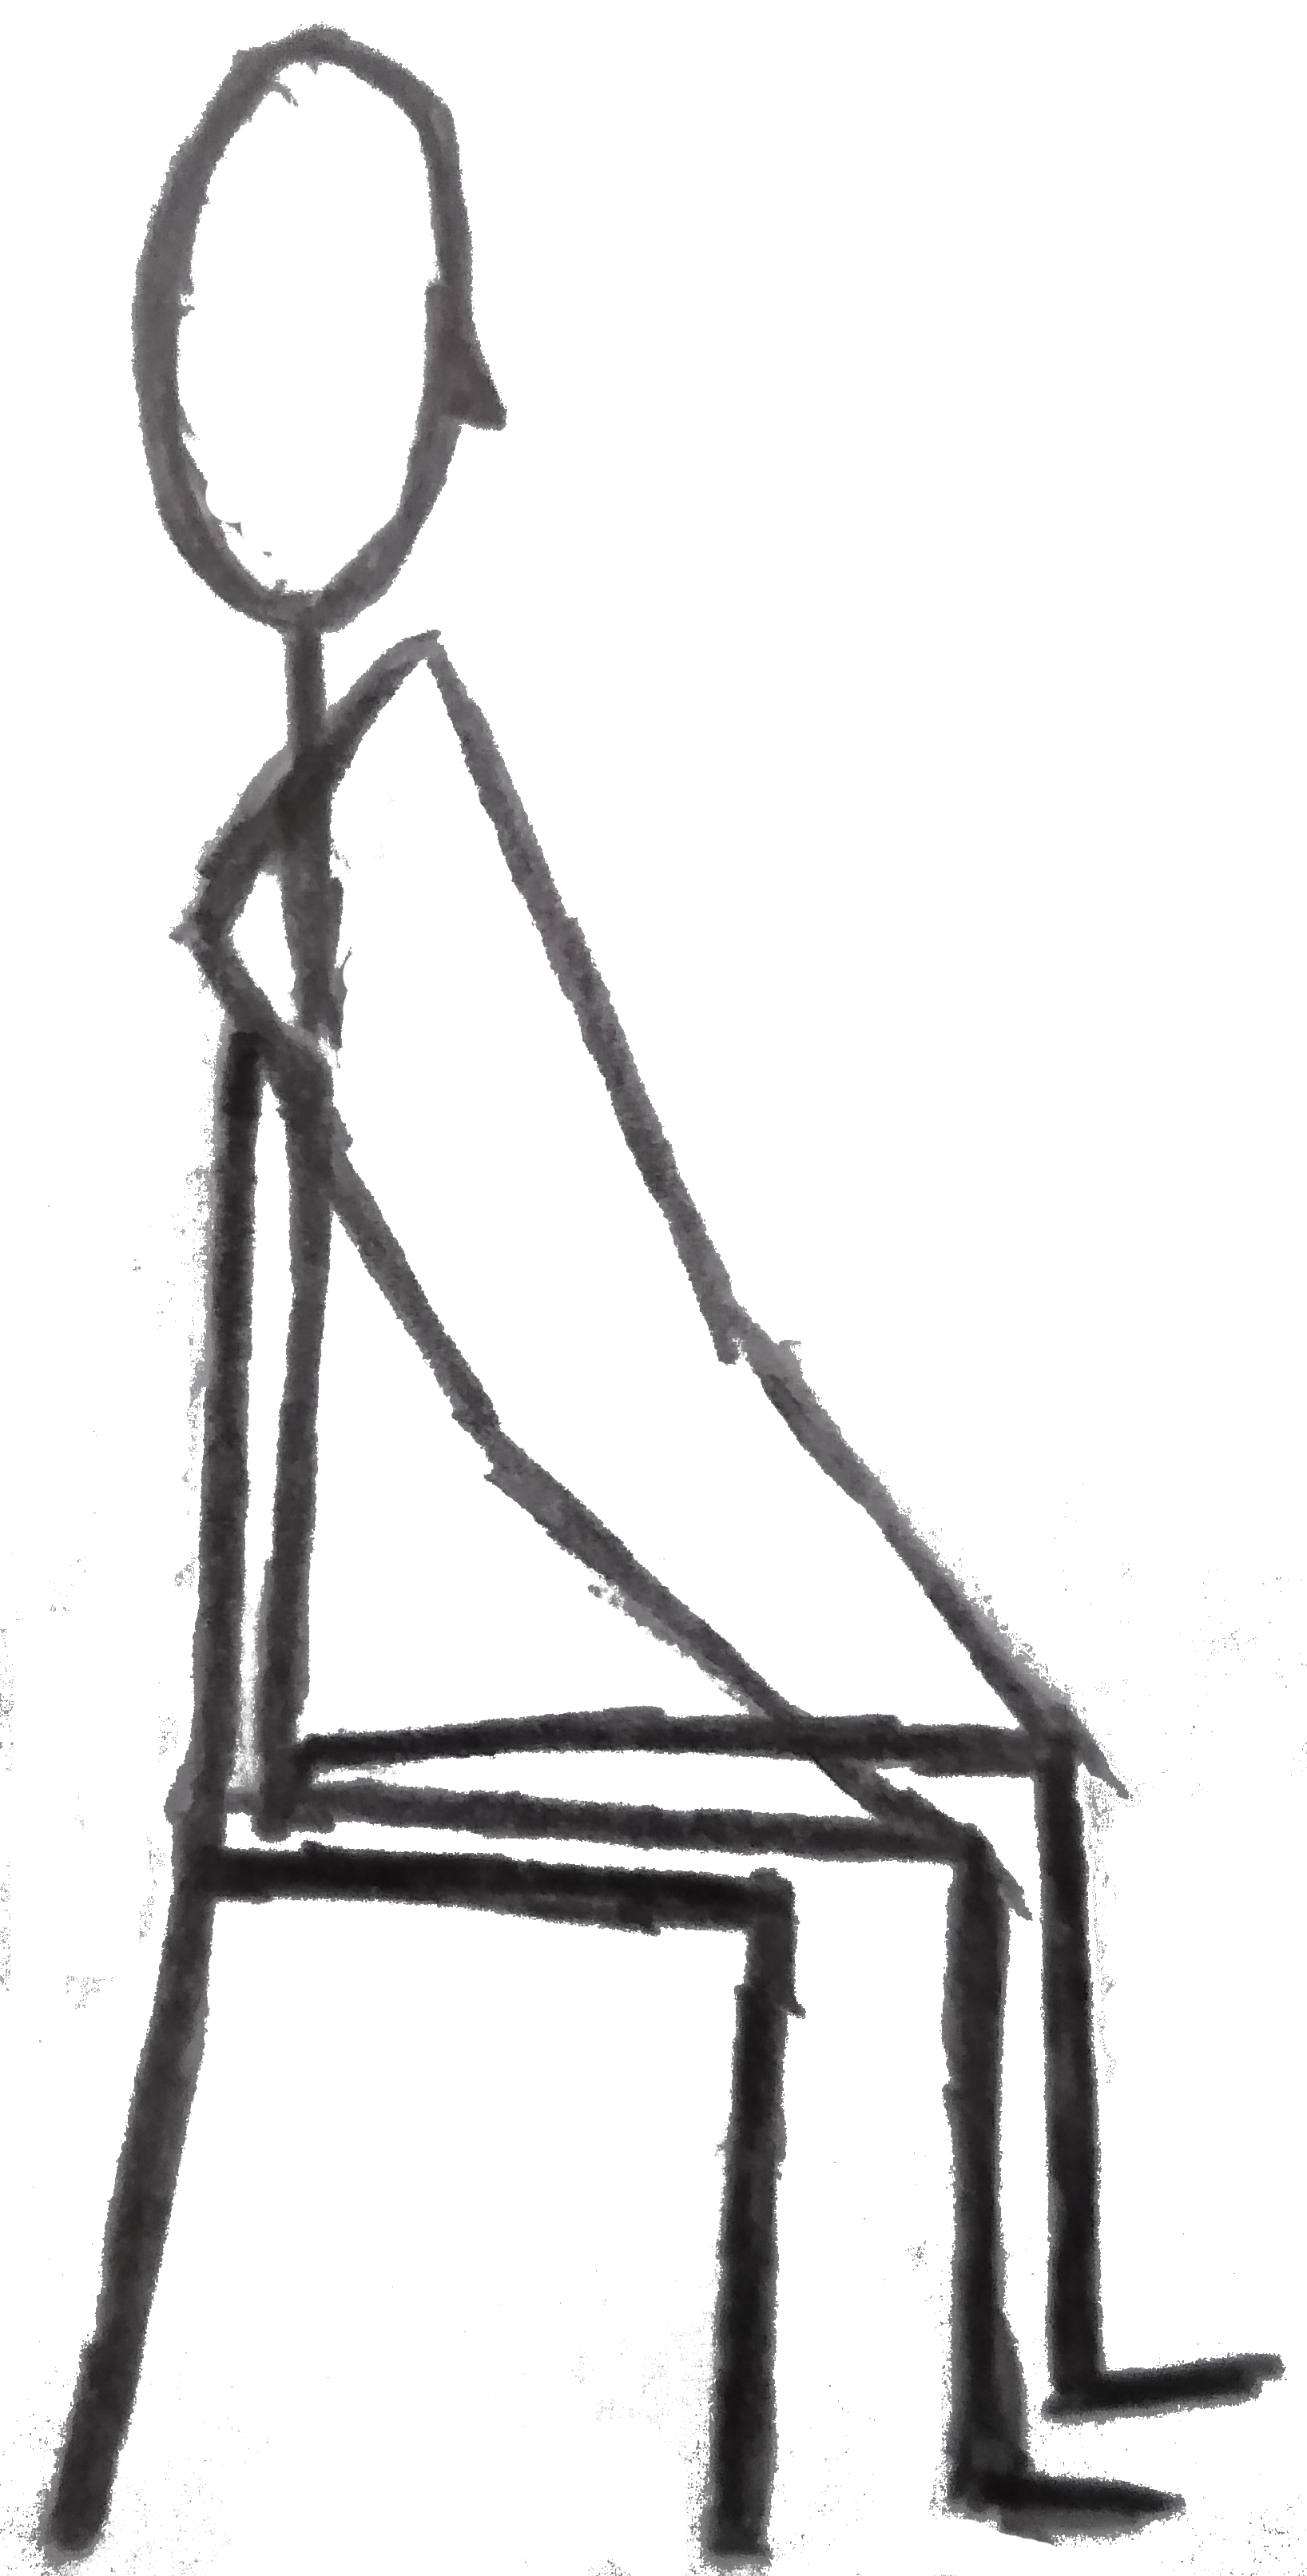
\includegraphics[width=\linewidth]{Sitting_chair_side.png}
%\column{.7\textwidth} % Right column and width

The vegetative nervous system is sectioned into three different nervous systems: \structure{the sympathetic, the parasympathetic and the enteric (intramural) nervous system}.

Functionally, the sympathetic and the parasympathetic nervous system act as \structure{antagonists}. That means it's actions on organs are the opposite. The \structure{sympathetic nervous system} puts the body in a state of \structure{heightened alertness} and ready for flight. The \structure{parasympathetic nervous system} on the other side regulates the functions down and puts the body in a \structure{state of rest}.

The vegetative and somatic nervous system \structure{collaborate very closely}. In some cells, it's impossible to distinguish their nervous cells from each other.
%\end{columns}
\end{frame}

%---------------------------------------------------------------
\begin{frame}
\frametitle{The enteric nervous system}
%\begin{columns}[c] % The "c" option specifies centered vertical alignment while the "t" option is used for top vertical alignment

%\column{.3\textwidth} % Left column and width
%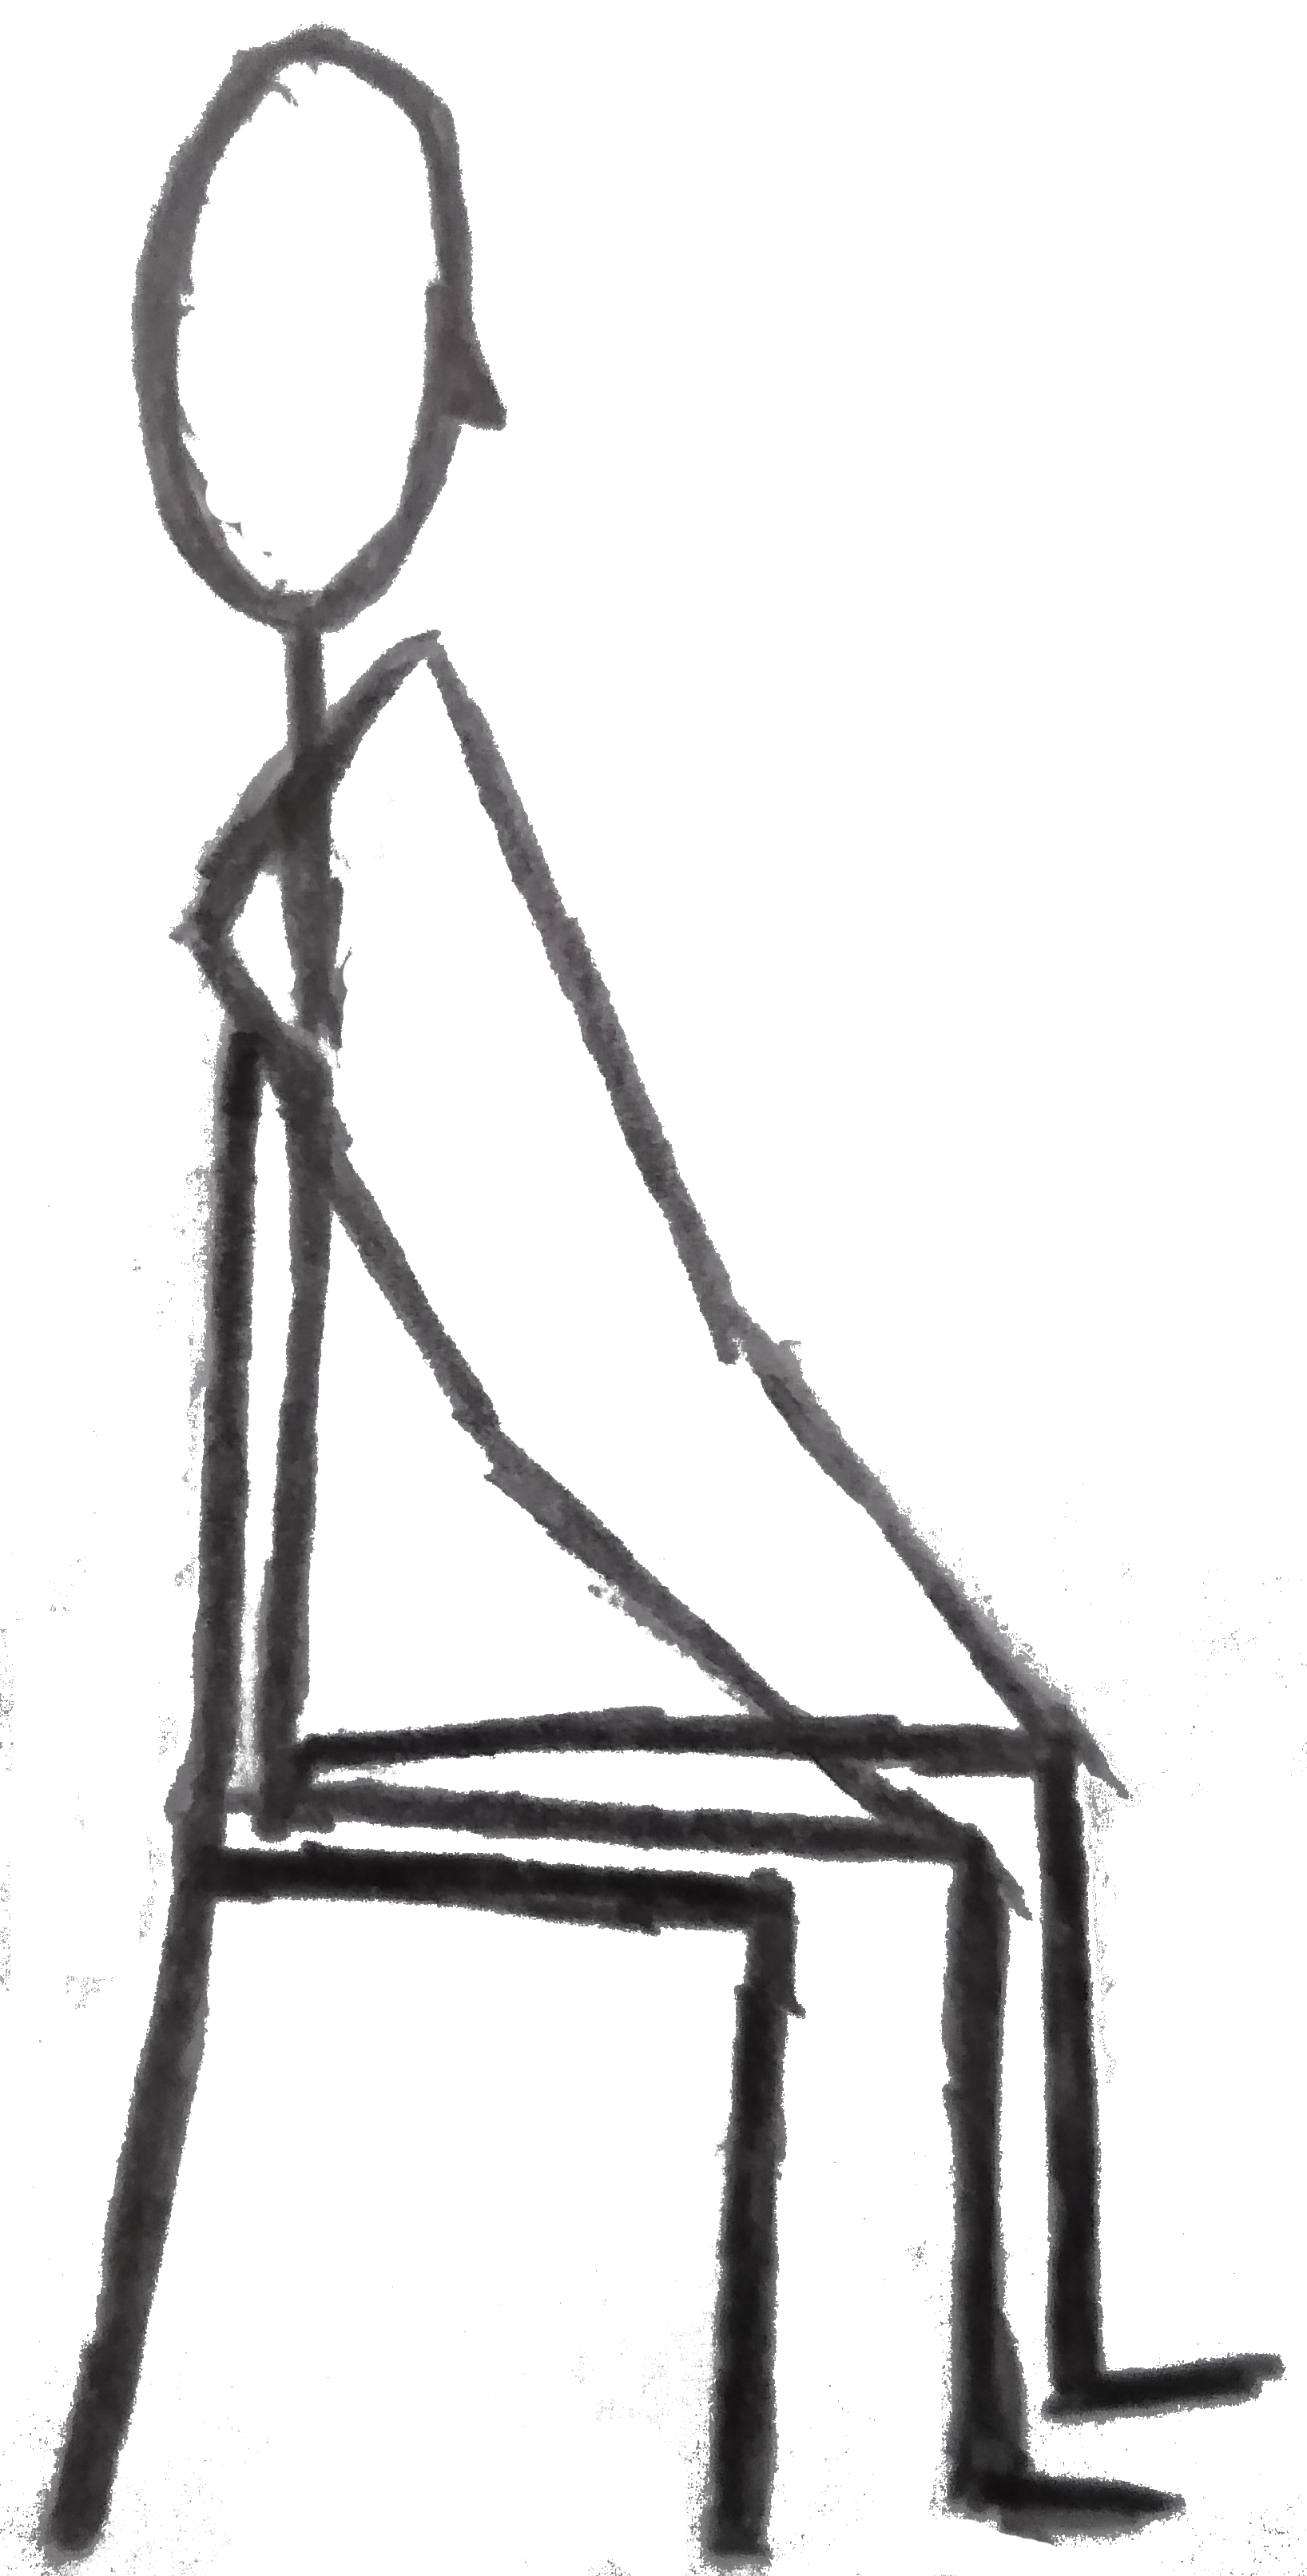
\includegraphics[width=\linewidth]{Sitting_chair_side.png}
%\column{.7\textwidth} % Right column and width

The enteric system consists of vegetative nervous fibers and ganglia in the \structure{walls of hollow organs} (heart, stomach, colon, bladder, uterus), which show a certain \structure{independence} in their operation. The nervous system in the \structure{walls of the colon} is part of the enteric nervous system and functions completely \structure{independent of the central nervous system} (brain and spine).

%\end{columns}
\end{frame}


%------------------------------------------------------------
\begin{frame}
\frametitle{References}
\begin{itemize}
\item[-] \url{https://en.wikipedia.org/wiki/Autogenic_training}
\item[-] \url{http://www.infotaste.com/moral-aspect-of-autogenic-training/}
\item[-] \url{https://psicoter.es/_arts/01_A166_01.pdf}
\item[-] \url{https://www.antimaximalist.com/autogenic-training/}
\item[-] Education material as a trainer for autogenous training, Swiss institute of stress research.
\end{itemize}
\end{frame}
%------------------------------------------------------------
